\section{Introduzione}

La valutazione del sisitema respiratorio con analogie elettriche permette di analizzare differenti quadri clinici per la fisiopatologia polmonare. 

Differenti autori attribuiscono al sistema polmonare diversi contributi inerziali ed elastici spesso traducibili in un modello elettrico di circuito RLC \cite{ghafarian_review_nodate}. In questo report vengono trascurati i contributi inerziali e si analizza un modello RC che permette di descrivere il sistema polmonare con buona approssimazione. 

L'introduzione di questi modelli in un software di simulazione permette di analizzare e modellare differenti comportamenti respiratori. 

Questo può essere integrato con la modellazione di un sistema di ventilazione a controllo di pressione imponendo la forma d'onda di pressione in ingresso all'apparato respiratorio. 

L'unione dei due modelli smulativi permette di studiare il rilevamento, diagnosi e trattamento di particolari patologie e analizzare come variano le risposte dell'apparato respiratorio al variare dei parametri del respiratore.

La necessità di supporto alla ventilazione è una frequente causa di trasferimento del paziente in unità di terapia intensiva e analizzare la complessa fisiolofia polmonare con modelli semplificate porterebbe ad una gestione migliore del paziente e dei dispositivi di ventilazione.

Inoltre, un sistema digitale di simulazione permette di analizzare meglio le curve di flusso verso le quali si trova sempre più interesse in clinica \cite{hamahata_go_2020}. Tali curve contengono molte informazioni sulla meccanica respiratoria, sullo sforzo del paziente e sulla modalità di ventilazione, parametri compresi. Analizzare correttamente tali curve permette di capire se il pattern respiratorio del paziente è sincronizzato con la macchina o se viene richiesto al paziente uno sforzo troppo elevato che potrebbe richiedere ventilazione prolungata o portare a danni polmonari gravi.

\section{Background}

Affinché sia possibile simulare correttamente il paziente è richiesta la scelta di un modello di meccanica respiratoria sufficientemente accurata e il fitting di tale modello sulle peculiarità del paziente.

Nella sezione seguente viene analizzato un modello per la meccanica respiratoria e confrontati alcuni parametri di resistenze e compliance evidenziati in letteratura come proprietà medie della popolazione.

Tale modello viene implementato in \texttt{Simulink} insieme a differenti forme d'onda di pressione. Successivamente viene affrontata anche la descrizione di un modello di ventilatore polmonare in  \texttt{Simulink} tale da permettere all'utente la personalizzazione dei parametri di ventilazione.



\subsection{Analogia circuitale}

\begin{figure*}[t!]
	\begin{subfigure}{0.5\linewidth}
		\centering
		\small{
			\def\svgwidth{\linewidth}
			\input{circuit.pdf_tex}}
		\caption{}
		\label{fig:modello}
	\end{subfigure}\hfill
	\begin{subfigure}{0.5\linewidth}
		\centering
		\small{
			\def\svgwidth{0.7\linewidth}
			\input{lung.pdf_tex}}
		\caption{}
	\end{subfigure}\hfill
	\caption{Analogia circuitale della meccanica respiratoria \cite{khoo_physiological_2018} (a); Rappresentazione schematica della divisione del circuito polmonare in due contributi resistivi (vie aeree superiori e inferiori) e in due contributi capacitivi (compliance del polmone e della parete toracica), raffigurate anche la pressione alveolare e pleurica.}
\end{figure*}

Il circuito polmonare può essere analizzando facendo un'analogia con i circuiti elettrici.

In particolare è possibile fare un parallelismo tra il flusso d'aria e la corrente elettrica (flusso di cariche) vedendo e la pressione come la presenza di un potenziale elettrico.
Si rivede allora la resistenza meccanica come il rapporto tra l'incremento di pressione rispetto il flusso, analoga alla resistenza elettrica. Similmente la compliance non è altro che il rapporto tra l'aumento di volume e l'aumento di pressione, in analogia elettrica è un condensatore.

Il sistema in \cref{fig:modello} è un modello di meccanica respiratoria che trascura la presenza di contributi inerziali (non ci induttanze) e considera la presenza di due compartimenti. Sono separate le vie aeree superiori, con il loro contributo resistivo $R_C$ dalle vie aeree inferiori $R_P$. I due compartimenti sono in serie tra loro ed in serie ai serbatoi d'aria, ovvero le capacità rappresentanti il contributo di compliance della parete $C_W$ e del polmone $C_L$. 
Tali contributi sono in serie proprio perché il volume d'aria passante è lo stesso. 

A questo si aggiunge anche la capacità di shunt $C_S$ che tiene conto di diversi contributi quali lo spazio morto anatomico, la deformabilità delle vie aeree e la comprimibilità dell'aria. Normalmente questo volume è molto piccolo in condizioni respiratorie normali (in assenza di patologie) e a basse frequenze respiratorie.

Si identificano allora anche le pressioni nei nodi. La pressione alle vie aeree $P_{aw}$, la pressione pleurica $P_{pl}$ e la pressione alveolare $P_A$. Chiaramente l'ingresso del sistema, dato dalla bocca e dalle cavità nasali, è rappresentato dalla pressione all'apertura delle vie aeree $P_{aO}$. 



\subsection{Risposta del sistema}

Il circuito in \cref{fig:modello} può essere descritto dalle seguenti equazioni:

\begin{equation}
	\footnotesize{
	\left\{\begin{array}{l}
		P_{a O}=Q R_{C}+\frac{1}{C_{S}} \int\left(Q-Q_{A}\right) \\
		\frac{1}{C_{s}} \int\left(Q-Q_{A}\right)=Q_{A} R_{P}+\left(\frac{1}{C_{L}}+\frac{1}{C_{W}}\right) \int Q_{A}
	\end{array}\right.}
\label{eq:modello}
\end{equation}

Si ottiene allora la funzione di trasferimento del sistema:

\begin{equation}
		\footnotesize{
\begin{aligned}
	H(s)&=\frac{Q(s)}{P_{a O}(s)}=\\
	&=\frac{s^{2}+s \frac{1}{R_{P}}\left(\frac{1}{C_{S}}+\frac{1}{C_{e q}}\right)}{s^{2}\left(R_{C}\right)+s\left(\frac{R_{C}+R_{P}+\frac{R_{C} C_{S}}{C_{e q}}}{C_{S} R_{P}}\right)+\frac{1}{C_{e q} C_{S} R_{P}}}
\end{aligned}}
\label{eq:fdt}
\end{equation}

Dove si esprime la serie delle capacità come: 

\begin{equation}
	{1\over C_{eq}}={1\over C_{L}}+{1\over C_{W}}
\end{equation}



\subsection{Proprietà del sistema}


Chiaramente la soluzione di tale problema richiede la conoscenza della meccanica polmonare propria del paziente. Si assume che il paziente abbia una meccanica polmonare normale.

I coefficienti numerici vengono selezionati da \citeauthor{khoo_physiological_2018} \cite{khoo_physiological_2018}, sono riportati in \cref{tab:coefficienti}.


\begin{table}[h!]
	\centering
	\begin{tabular}{|c|c|c|}
		\hline
		Parametro & Valore & Unità \\ \hline
		$R_C$ & 1 & cm H\textsubscript{2}O s / L \\ \hline
		$R_P$ & 0.5 & cm H\textsubscript{2}O s / L \\ \hline
		$C_L$ & 0.2 & L / cm  H\textsubscript{2}O \\ \hline
		$C_W$ & 0.2 & L / cm  H\textsubscript{2}O \\ \hline
		$C_S$ & 0.005 & L / cm  H\textsubscript{2}O \\ \hline
	\end{tabular}
\caption{Coefficienti numerici per il sistema \cite{khoo_physiological_2018}}
\label{tab:coefficienti}
\end{table}

\subsection{Modellazione del sistema}

La risoluzione del sistema richiede la risoluzione di una ODE e l'approccio, quando le equazioni diventano complesse, è quello di trasferire il modello in un calcolatore. Il classico approccio è di tipo numerico, mediante l'utilizzo di un codice numerico di risoluzioni.

Esiste tuttavia la possibilità di utilizzare  \texttt{Simulink}. 

\subsection{Simulink}


 \texttt{Simulink} \cite{simulink} è un software sviluppato da MathWorks che fornisce un approccio grafico basato su un ambiente che permette all'utente di convertire il problema in una rete di blocchi di funzioni matematiche. 

Inoltre, tale ambiente permette l'integrazione con l'ambiente di Matlab e le relative funzioni di programmazione. 

Un primo approccio sintetico potrebbe essere quello di diagrammare un sistema ingresso-uscita per il tramite della funzione di trasferimento in \cref{eq:fdt}. Tale modello risulterebbe però troppo sintetico e non permetterebbe l'accesso ad alcune variabili esterne, come i singoli flussi.

Si sceglie allora di modellare il sistema completo in \cref{eq:modello}. Tale sistema viene modellato nel blocco \texttt{lungs}. Vengono poi aggiunti anche un sotto sistema per simulare un ventilatore polmonare, ovvero l'ingresso come $P_{aO}$, e un blocco per visualizzare e salvare i dati.

Uno schema generale di alto livello è presente in \cref{fig:generale}


\subsubsection{Sotto sistema del ventilatore}


\begin{figure*}[t!]
	\centering
	\begin{subfigure}{0.4\linewidth}
		\centering
		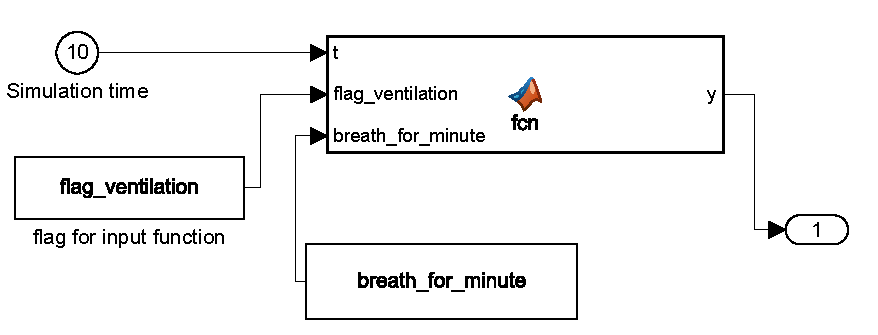
\includegraphics[width=\linewidth]{simulink_ventilator.pdf}
		\caption{}
	\end{subfigure}\hfill
	\begin{subfigure}{0.6\linewidth}
		\centering
		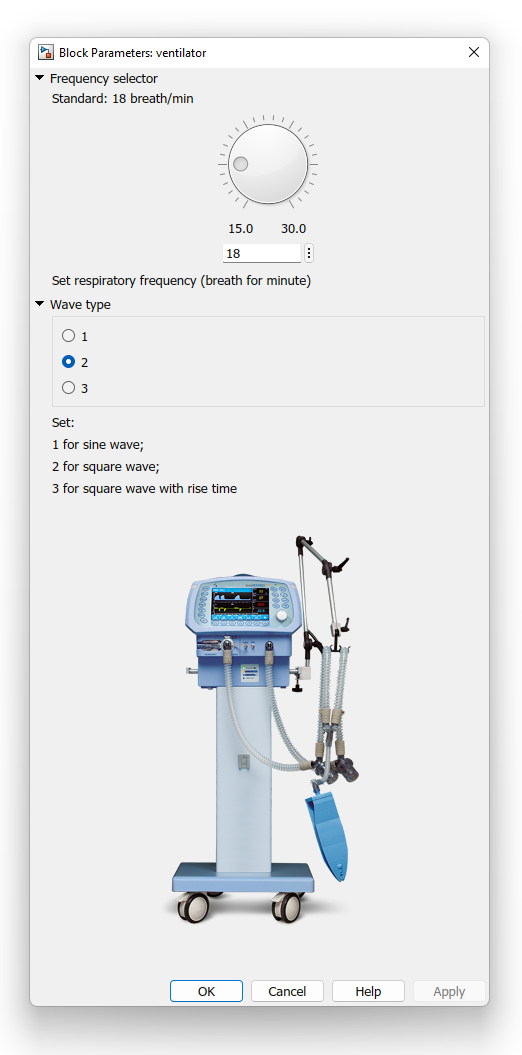
\includegraphics[angle=90,width=0.95\linewidth]{simulink_ventilator_GUI}
		\caption{}
		\label{fig:mask}
	\end{subfigure}\hfill
	\caption{Sistema di input rappresentante il ventilatore: schema a blocchi  \texttt{Simulink} dove il segnale di ingresso ($P_{aO}$) viene generato tramite una funzione (\text{fcn}) Matlab (a); GUI tramite la quale è possibile selezionare la frequenza respiratoria e selezionare la forma d'onda.}
\end{figure*}


Nel sotto sistema del ventilatore l'obiettivo è di fornire una $P_{aO}$ con una forma d'onda precisa. Vengono fornite diverse forme d'onda e la frequenza stessa, in atti respiratorio per minuto, può essere variata.

Per fare questo si utilizza un blocco \texttt{funzione Matlab} mediante il quale si può definire un codice Matlab contente la forma d'onda della pressione al variare del tempo di input. Maggiori informazioni sono riportare in appendice. 

Tale blocco richiede anche due variabili ausiliare tramite le quali è possibile scegliere la frequenza respiratoria e il tipo di forma d'onda direttamente dall'interfaccia grafica della maschera del blocco (\cref{fig:mask}). Tramite la maschera di blocco viene anche settata una funzione di callback che permette di aggiornare il nome del file di output, non appena vengono cambiati i parametri, con una struttura del tipo:
\begin{equation*}
	\text{"forma d'onda } + \text{ frequenza } + \text{ .mat"}
\end{equation*}


\subsubsection{Sotto sistema del polmone}


\begin{figure*}[t!]
	\centering
	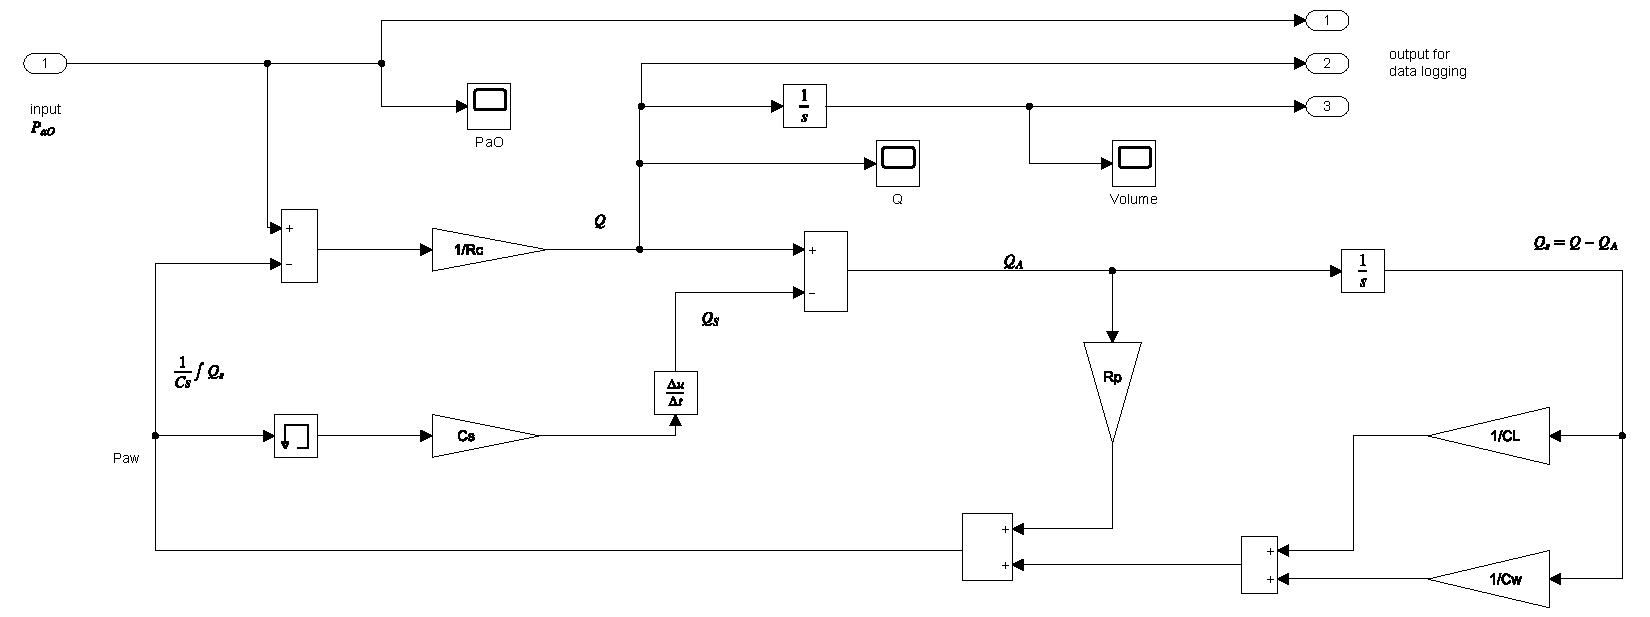
\includegraphics[width=\linewidth]{simulink_lung.pdf}
	\caption{Modello del blocco in  \texttt{Simulink} rappresentante il circuito polmonare (in \cref{eq:modello}, \cref{fig:modello})}
	\label{fig:simulinkLung}
\end{figure*}

Le equazioni descrittive del sistema (\cref{eq:modello}) e i relativi segmenti circuitali possono essere rappresentati direttamente nel modello  \texttt{Simulink} in \cref{fig:simulinkLung}. 

Tramite la modellazione in  \texttt{Simulink} è possibile sommare i contributi di segnale (rappresentanti segmenti del circuito o, equivalentemente, membri dell'equazione), moltiplicare per un costante applicando un guadagno al segnale, derivare e integrare. 
Chiaramente, per passare dal flusso al volume è sufficiente integrare nel tempo. 

Sono presenti anche 3 blocchi di tipo \texttt{scope} per visualizzare le forme d'onda direttamente all'interno della simulazione, il blocco di ingresso (prende il segnale $P_{aO}$ direttamente dal ventilatore) e i 3 blocchi di output utilizzare per salvare i dati. 


\section{Risultati}

\subsection{Ventilazioni ideali}

Un approccio semplice, per analizzare la meccanica polmonare, è quello di ventilare con una forma d'onda ideale. Si utilizza come prima analisi una forma sinusoidale di ampiezza di 2.5 cm H\textsubscript{2}O (ampiezza picco-picco di 5 cm H\textsubscript{2}O) con una frequenza di 15 respiri al minuto \cite{khoo_physiological_2018}, simile alla respirazione a riposo.

Dai grafici in \cref{fig:sine_wave_15} è possibile vedere come il volume segue un andamento simile, seppur leggermente sfasato. Questo è indice che, a bassa frequenza, l'andamento è dominato dal contributo di compliance (dove c'è proporzionalità con l'integrale del flusso). L'ampiezza di picco del volume raggiunge 0.5 L e il flusso circa 0.7 L/s. L'andamento del flusso invece è significativamente sfasato rispetto il contributo di pressione in ingresso. 

\begin{figure*}[t!]
\begin{subfigure}{0.5\linewidth}
	\centering
	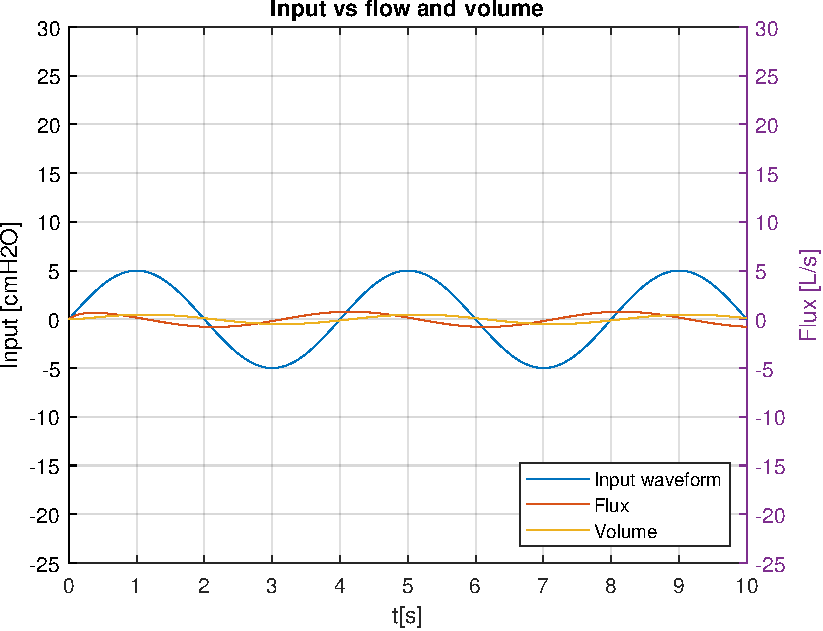
\includegraphics[width=0.95\linewidth]{../model/data_log/data_sine_wave_freq_15.pdf}
	\caption{}
\end{subfigure}\hfill
\begin{subfigure}{0.5\linewidth}
	\centering
	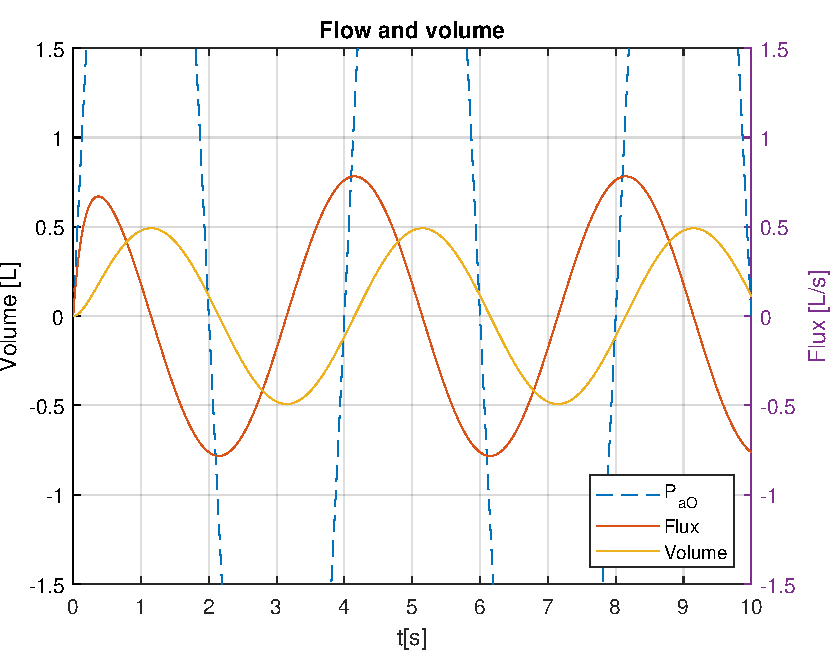
\includegraphics[width=0.95\linewidth]{../model/data_log/data_sine_wave_freq_15_zoom.pdf}
	\caption{}
\end{subfigure}
\caption{Confronto tra la pressione in ingresso con forma d'onda sinusoidale ideale con l'andamento del flusso e del volume (a); ingrandimento sull'andamento di flusso e volume (b). Si può osservare come volume e sfasamento presentano uno sfasamento di 90°. Inoltre, ne flusso ne volume sono in fase con l'andamento della $P_{aO}$. }
\label{fig:sine_wave_15}
	\centering
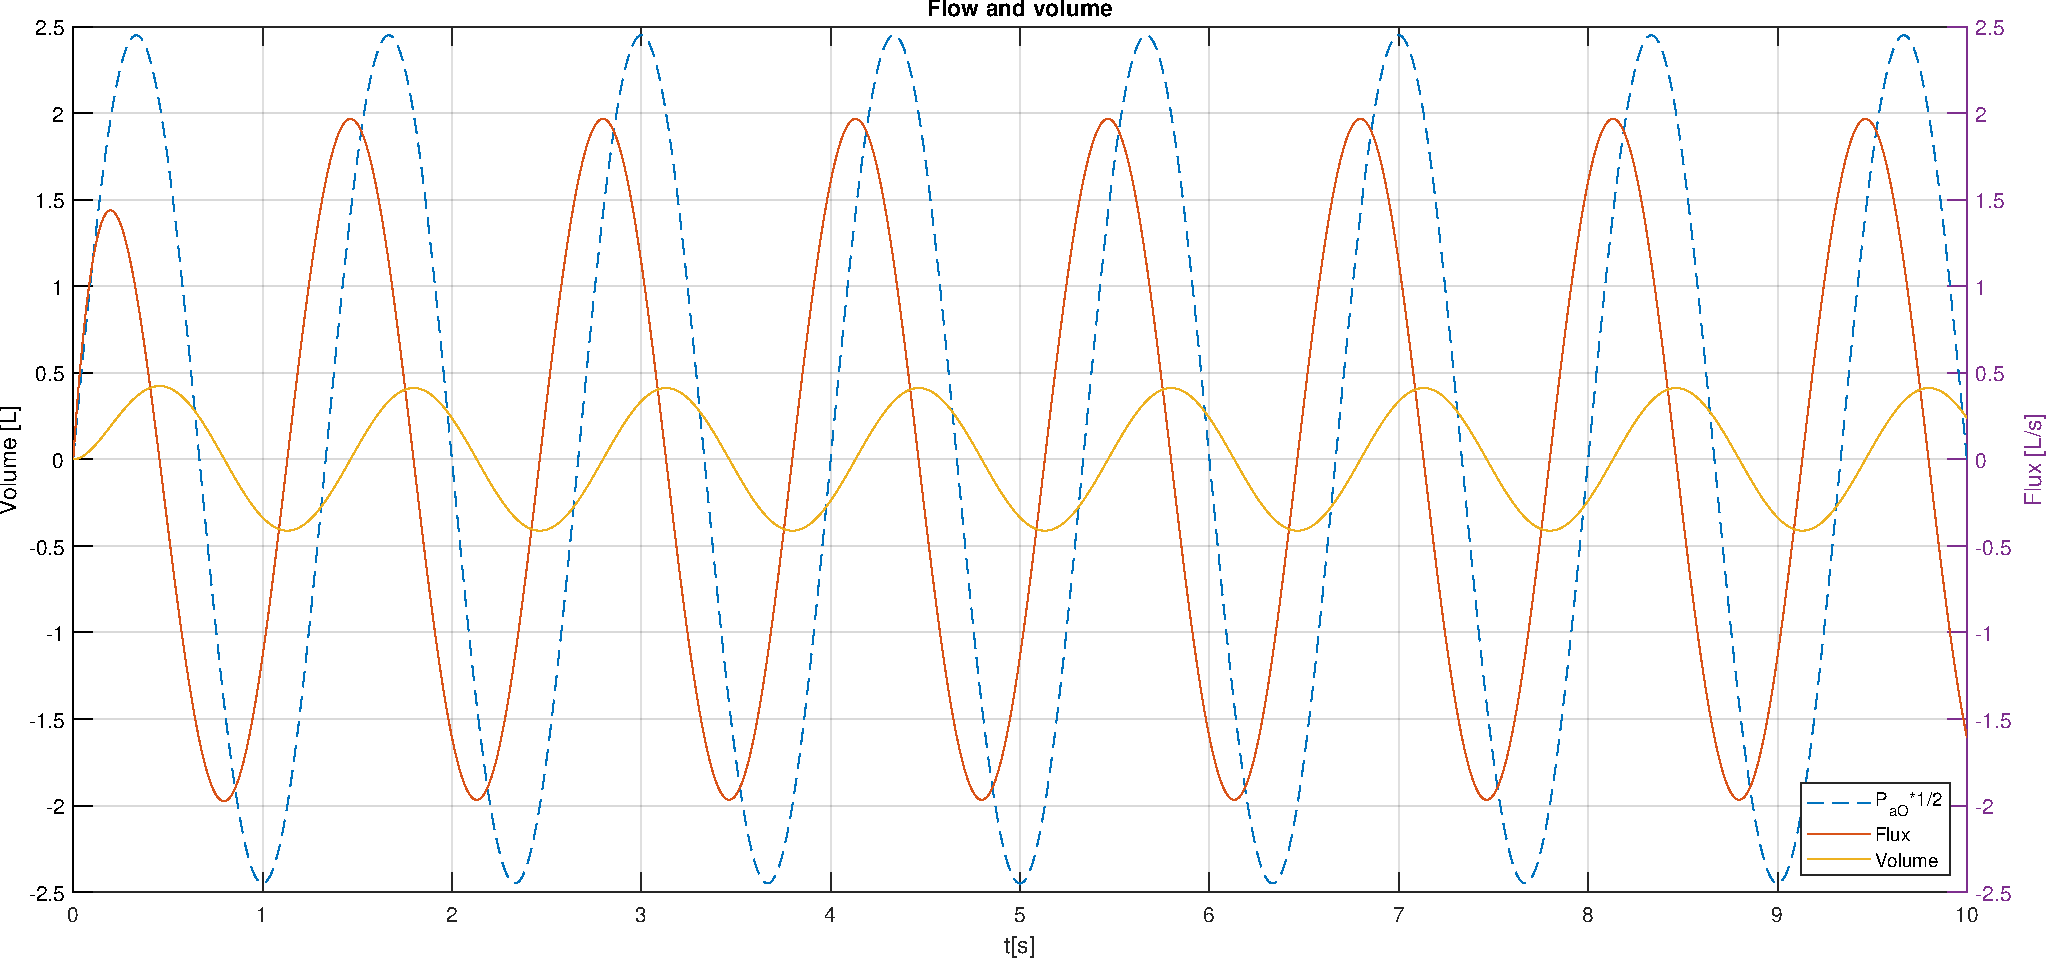
\includegraphics[width=0.95\linewidth]{../model/data_log/data_sine_wave_freq_45_zoom.pdf}
\caption{Andamento di flusso, volume e $P_{aO}$. L'ampiezza della $P_{aO}$ è scalata di un fattore $1/2$. Per la curva del flusso si osserva una riduzione delle sfasamento e un aumento dell'ampiezza di picco.Il volume tende a ridursi (rispetto al caso 15 respiri/min) simbolo di un comportamento più rigido del polmone.}
\label{fig:sine_wave_45}
\end{figure*}

Aumentando la frequenza, triplicando il numero di respiri al minuto (\cref{fig:sine_wave_45}), il polmone appare più rigido e infatti l'ampiezza del volume tende a ridursi nonostante aumenti il flusso. L'ampiezza di picco del volume passa da 0.5 L a 0.4 L sebbene il flusso sia passato da 0.7 L/s a quasi 2 L/s. Questo rappresenta come nonostante il ricambio d'aria sia maggiore il polmone per aumentare la frequenza respiratoria è costretto ad espandersi meno limitando l'introito complessivo di aria.   

Inoltre, l'andamento del volume tende a sfasarsi maggiormente rispetto l'andamento della pressione mentre il flusso sembra essere più in fase, simbolo di un maggior contributo di tipo resistivo (proporzionalità diretta pressione-flusso).

Quindi, mentre a bassa frequenza (riposo) il contributo è maggiormente legato alla compliance, ad alta frequenza il comportamento resistivo sembra essere maggiormente presente.
\\

Una forma d'onda alternativa è l'onda quadra. Si può impostare una forma d'onda con ampiezza di picco equivalente alla precedente. Si osserva una risposta del sistema differente.

\begin{figure*}[t!]
	\begin{subfigure}{0.5\linewidth}
		\centering
		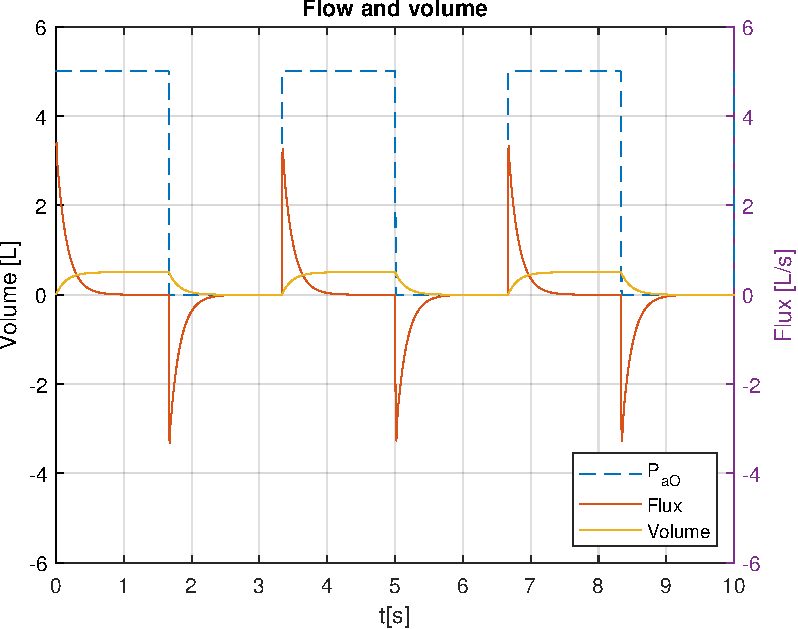
\includegraphics[width=0.95\linewidth]{../model/data_log/data_square_wave_freq_18.pdf}
		\caption{}
	\end{subfigure}\hfill
	\begin{subfigure}{0.5\linewidth}
		\centering
		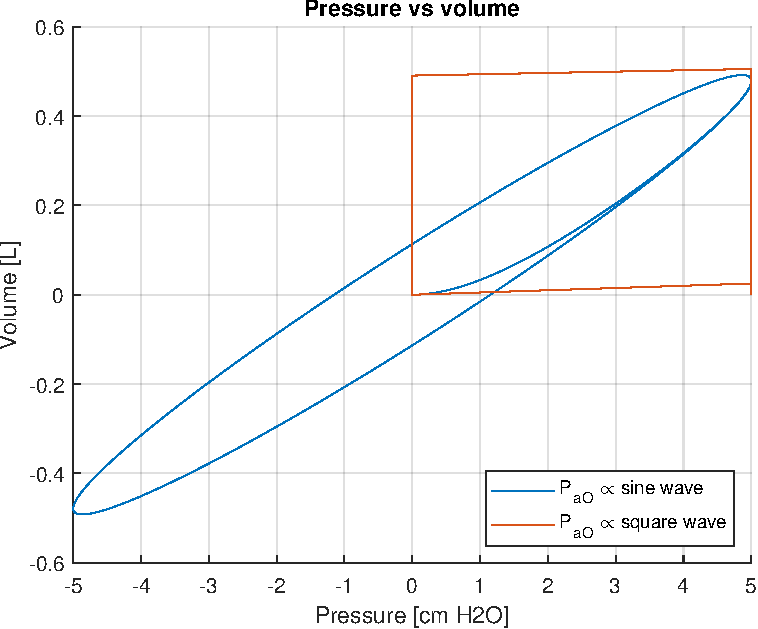
\includegraphics[width=0.95\linewidth]{../model/data_log/PV_sine_vs_square.pdf}
		\caption{}
	\end{subfigure}
	\caption{Andamento di flusso e volume rispetto l'ingresso di $P_{aO}$ come onda quadra con una frequenza di 18 respiri/min (a); grafico pressione-volume per ingresso sinusoidale e ad onda quadra)}
	\label{fig:square_wave_45}
\end{figure*}

Si osserva come il flusso torna rapidamente a zero e inizia una fase di plateau del volume. Successivamente inizia la fase inspiratoria dove il flusso presenta una curva simmetrica ma negativa con un picco della stessa ampiezza e il volume esce gradualmente. 

Inoltre, variando la frequenza il comportamento della curve di flusso e di volume non cambia ma si riduce la fase di plateau del volume. 
\\

Chiaramente tale forme d'onda sono modelli analitici che nell'applicazione reale presenterebbero diversi problemi. Nella pratica clinica non si utilizzano mai pressioni negative ma si mantiene sempre un gradiente di pressione positivo per cui tali curve sono da escludere per casi applicativi realistici. Si osservi anche come la stessa presenza di un volume negativo, nella forma d'onda sinusoidale, non è desiderabile per un ventilatore il cui scopo è aiutare il paziente a respirare riducendo il lavoro respiratorio del polmone o sostituendolo completamente.

\subsection{Ventilazione a controllo di pressione}

Le analisi precedente sono utili per capire il modello matematico e per avere un'idea di base sulla meccanica respiratoria. Tuttavia, in clinica, l'approccio alla ventilazione è leggermente differente. 

Al fine di realizzare un simulatore digitale di un ventilatore polmonare si considera una forma d'onda tipicamente diffusa in clinica per la ventilazione a controllo di pressione \cite{al-naggar_modelling_2015}. 

La ventilazione polmonare assistita si divide in due macro categorie: controllo di volume e controllo di pressione. Sono presenti diversi vantaggi/svantaggi in entrambe e la scelta si basa su diverse considerazioni paziente specifiche. Nella ventilazione a controllo di pressione (VCP) si imposta un target specifico, la pressione alle vie aeree $P_{aO}$ e il ventilatore deve mantenerla. A seconda del macchinario utilizzato possono essere variati alcuni parametri quali la percentuale di ossigeno, il volume tidale o la ventilazione per minuto, la frequenza respiratoria, il tempo inspiratorio, il flusso o settare dei valori limite per la pressione \cite{grossbach_overview_2011}.

Una curva generica, tipica della VCP, è costituita da un'onda quadra con un offset positivo che prende il nome di PEEP, positive end-expiratory pressure. Il periodo $T=\frac{1}{\text{freq. respiratoria}}$ è composto da un tempo di inspirazione e un tempo inspirazione. Facoltativamente può essere presente un certo tempo di salita, espresso in funzione del tempo di inspirazione \cite{al-naggar_modelling_2015}. 

Questo può essere espresso come una curva lineare a tratti (\cref{fig:PCV}) di periodo $T=T_{insp}+T_{esp}$:

\begin{equation}
	\small{
	P(t)=\left\{\begin{array}{c}
		P_{aO} \cdot \frac{t}{\tau}+\mathrm{PEEP} \\
		P_{aO}+\mathrm{PEEP} \\
		\mathrm{PEEP}
	\end{array}\right.\quad \begin{aligned}
		&0 \leq t < \tau \\
		&\tau \leq t < T_{insp} \\
		&T_{insp} \leq t 
	\end{aligned}}
\end{equation}

 \begin{figure*}[t!]
	\begin{subfigure}[b]{0.5\linewidth}
		\centering
		\footnotesize{
			\def\svgwidth{\linewidth}
			\input{PCV_VCV.pdf_tex}}
		\caption{}
	\end{subfigure}\hfill
	\begin{subfigure}[b]{0.5\linewidth}
		\centering
		\footnotesize{
			\def\svgwidth{\linewidth}
			\input{PCV.pdf_tex}}
		\caption{}
		\label{fig:PCV}
	\end{subfigure}
	\caption{Differenza tra le curve ottenute in ventilazione a controllo di pressione (VCV) e a controllo di pressione (PCV) (a); generica forma d'onda per la ventilazione a controllo di pressione (b)}
	\label{fig:clinical}
\end{figure*}

La PEEP generalmente si mantiene tra $5\div 10$ cmH\textsubscript{2}O mantenendo il volume nel range di $4\div 6$ ml/kg di peso corporeo. La $P_{aO}$ viene mantenuta sotto i 35 cm H\textsubscript{2}O \cite{ball_modes_2015,article}.

A tal proposito viene anche modificata l'interfaccia grafica (\cref{fig:mask}) in moto tale da permette la selezione di una forma d'onda di tipo onda quadra con un rise time e un offset di pressione, lasciando all'utente la possibilità di scegliere frequenza, tempo di inspirazione (in funzione del periodo), rise time (in funzione del tempo di inspirazione), $P_{aO}$ e $\mathrm{PEEP}$. L'interfaccia completa è presente in appendice (\cref{fig:interfaccia})
 


Una volta impostato tale simulatore permette di calibrare la ventilazione e di addestrarsi nell'utilizzo di un ventilatore reale andando a vedere come i diversi parametri di ventilazione influenzano la meccanica respiratoria e soprattutto come modificare la ventilazione in base alla risposta del paziente.
\\

Nelle sezioni successive vengono fissati i parametri di ventilazione \cite{truwit_modes_2011} ad una frequenza di 18 respiri/min, un tempo di inspirazione del 30\% e un rise time del 15\%, con una $\mathrm{PEEP}$ di 5 cm H\textsubscript{2}O e una $P_{aO}=25$  cm H\textsubscript{2}O Questi parametri permettono di approssimare le forme d'onda tipicamente utilizzate in clinica \cite{al-naggar_modelling_2015}. 

Al fine di soddisfare la risposta del polmone, in termini di volume tidale \cite{ventilation_2000}, è necessario soddisfare una compliance complessiva del polmone di circa:

\begin{equation}
	C_{T}=\left({1 \over C_{W}}+{1 \over C_{L}}\right)^{-1}\approx 10 \text{ mL/cmH2O}
\end{equation}

Allora segue l'analisi considerando dei parametri medi di un'ordine di grandezza inferiore: $C_w=0.02$ L/cmH\textsubscript{2}O e $C_L=0.02$ L/cmH\textsubscript{2}O .

Si analizza allora come varia la ventilazione in funzione della variazione dei parametri del paziente. 

 \begin{figure*}[t!]
	\begin{subfigure}{0.5\linewidth}
		\centering
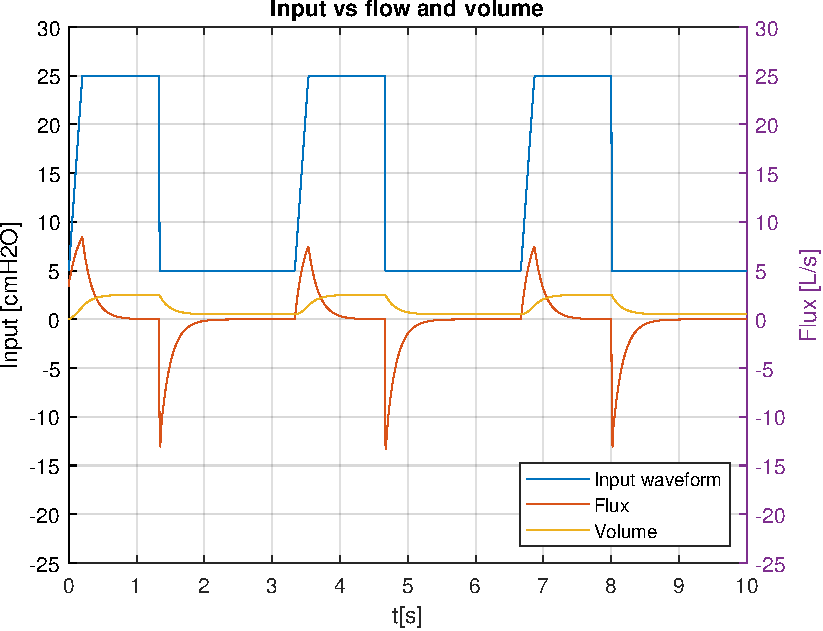
\includegraphics[width=0.95\linewidth]{../model/data_log/data_square_wave_rise_15_Tinsp_40_PEEP_5_Paw_25_freq_18}
		\caption{}
	\end{subfigure}\hfill
	\begin{subfigure}{0.5\linewidth}
		\centering
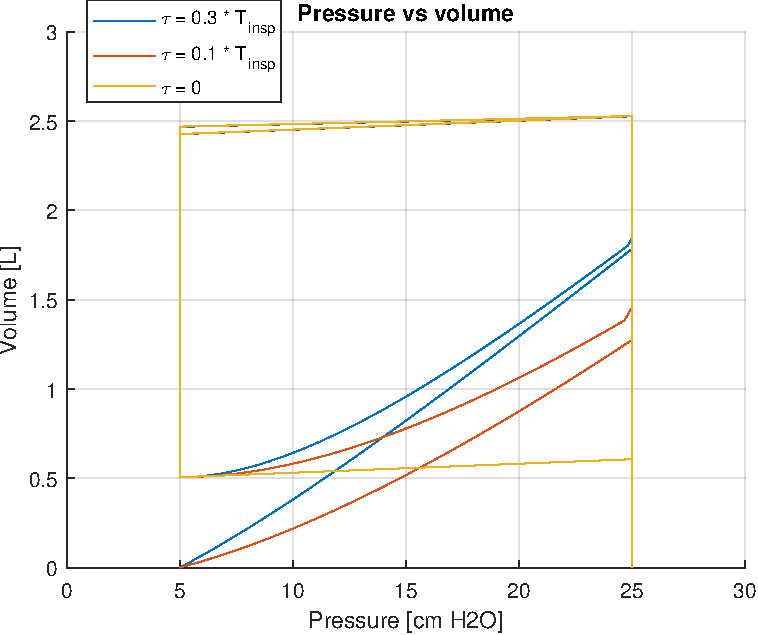
\includegraphics[width=0.95\linewidth]{../model/data_log/PV_rise_time.pdf}
		\caption{}
	\end{subfigure}
	\caption{PCV con $T_{insp}=0.4*T$, $f=$18 respiri/min, $\tau=0.15*T_{insp}$, $\mathrm{PEEP}=5$ cm H\textsubscript{2}O e $P_{aO}=25$ cm H\textsubscript{2}O (a); diagramma PV di confronto con differenti tempi di salita, si osserva come varia il primo ramo di salita del volume, riducendo il rise time l'incremento di volume diventa sempre più brusco ma il volume massimo raggiunto è sempre lo stesso.}
	\label{fig:rise_time}
\end{figure*}

\subsection{Resistenza delle vie aeree}

Esistono diverse patologie e quadri clinici che si traducono in un aumento delle resistenze delle vie aeree interne. 

Un aumento delle resistenze può essere causato da alterazioni istologiche, nella geometria alveolare o nell'alterazione dell'interfaccia aria-liquido.

Il lavoro muscolare che deve essere generato dai muscoli respiratori è dipendente dalle proprietà elastiche e resistive del sistema respiratorio per tutto l'intervallo coperto dalla variazione del volume. Normalmente il polmone presenta na compliance di circa 200 ml/cm H\textsubscript{2}O, ovvero quando la pressione transpolmonare (differenza tra la pressione negli alveoli e quella pleurica) aumenta di 1 cm H\textsubscript{2}O allora il polmone si espande di 0.2 L. Chiaramente, più piccola è la compliance più grande sarà la pendenza nel diagramma pressione-volume. 

La forza elastica è il maggior contributo (> 2/3 del totale) nel far collassare il polmone a causa della tensione superficiale all'interno degli alveoli. Sebbene questo non sia un problema nel polmone sano, diventa un problema nei casi in cui si riduce la quantità di surfractante polmonare, come ad esempio nella sindrome da distress respiratorio acuto (ARDS) \cite{milic-emili_basics_1999}, in cui la compliance diminuisce. 

L'enfisema è caratterizzato da un aumento della resisitenza respiratoria e un calo della compliance polmonare \cite{milic-emili_basics_1999}.

Sono presenti anche diversi fattori non legati a patologie specifiche che tendono ad aumentare le resistenze come la presenza di ostruzioni nel tubo endotracheale, tosse, secrezioni, broncospasmi e ritmo respiratori accelerato \cite{grossbach_overview_2011}.

A questo si aggiungono anche dei fattori esterni che possono variare sia la resistenza che la compliance come restrizioni dell'impianto di ventilazione, contrazione addominale o aumento della pressione addominale oppure danni o deformazioni della parete toracica.
\\

Si vede come, variando entrambe le resistenze presenti, la risposta del volume è quasi nulla. Invece, il flusso varia leggermente il picco raggiunto. Dalle \cref{fig:Rc_flux,fig:Rc_volume,fig:Rp_flux,fig:Rp_volume} si vede come il flusso è più sensibile alla variazione di $R_c$.

Ricordando che i test sono effettuati a parità di pressione, un aumento di resistenza si tradurrà in una riduzione del flusso. 

\begin{figure*}[t!]
\begin{subfigure}{\linewidth}
\centering
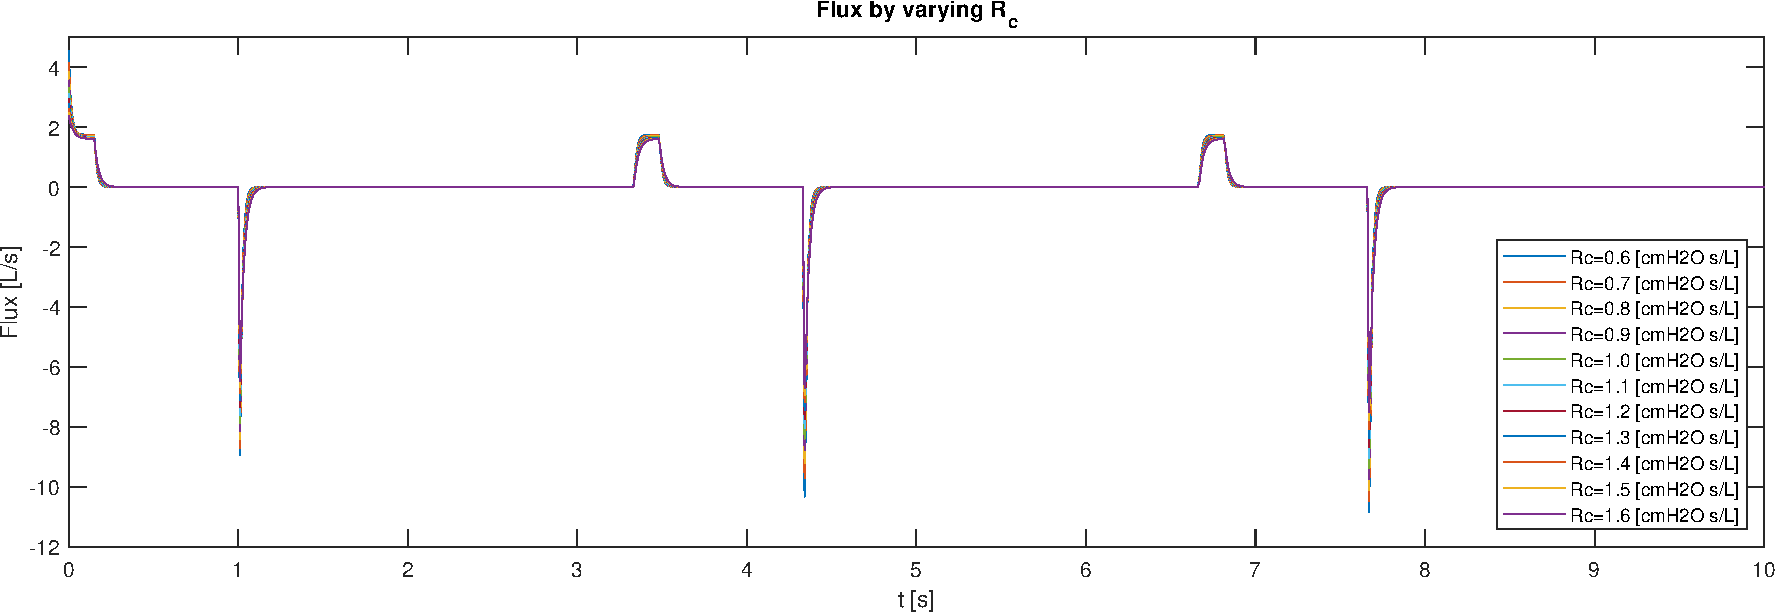
\includegraphics[width=0.95\linewidth]{../model/data_log/Rc_flux_total.pdf}
\caption{}
\end{subfigure}\hfill
\begin{subfigure}{0.5\linewidth}
	\centering
	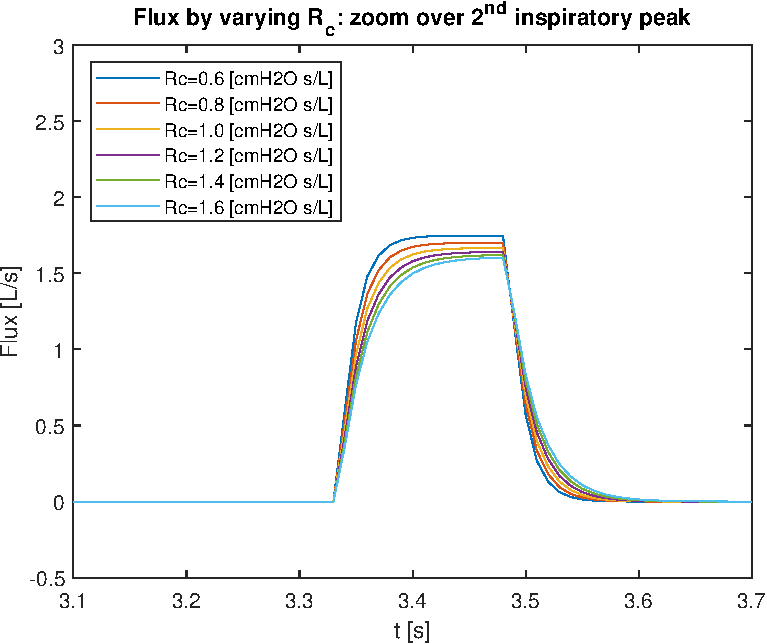
\includegraphics[width=0.95\linewidth]{../model/data_log/Rc_flux_zoom1.pdf}
	\caption{}
\end{subfigure}\hfill
\begin{subfigure}{0.5\linewidth}
	\centering
	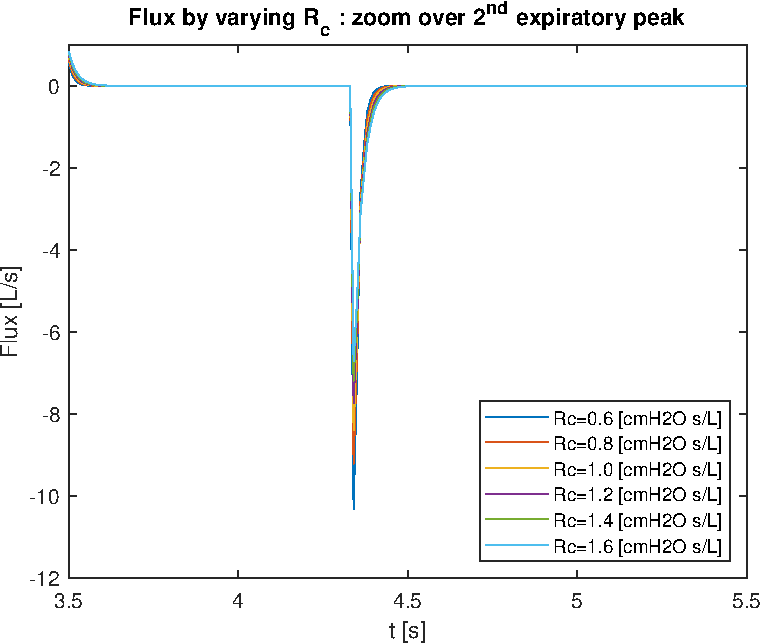
\includegraphics[width=0.95\linewidth]{../model/data_log/Rc_flux_zoom2.pdf}
	\caption{}
\end{subfigure}\hfill
\caption{Flusso con variazione della resistenza delle vie aeree superiori $R_c$ nel range $0.6\div 1$ [cmH\textsubscript{2}O s/L]. Flusso nel tempo (a); zooma nel secondo periodo respiratorio sulla zona di influsso (b) ed efflusso (c). Si vede come al ridursi della resistenza aumenta la velocità di variazione e il picco massimo.}
\label{fig:Rc_flux}
\vspace{0.8 cm}
\begin{subfigure}{0.7\linewidth}
	\centering
	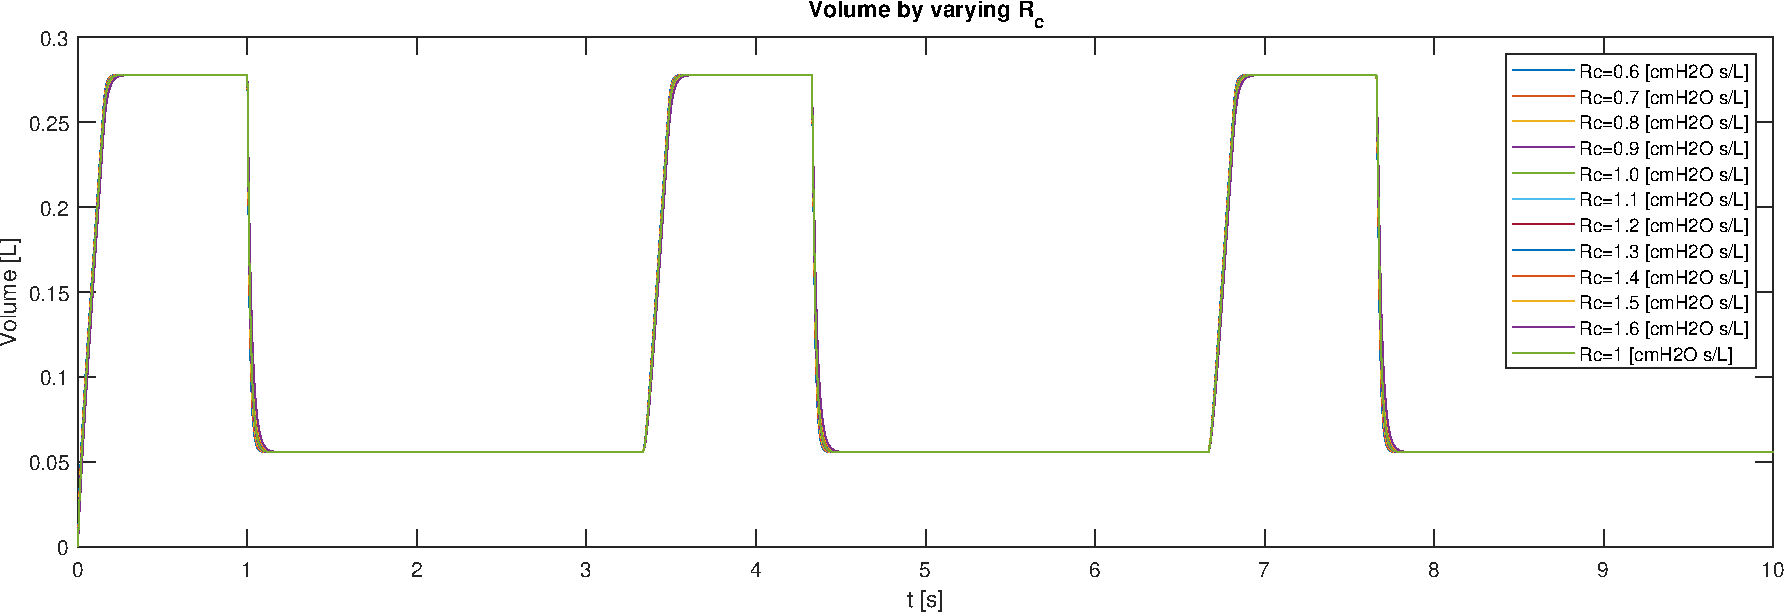
\includegraphics[width=0.95\linewidth]{../model/data_log/Rc_volume_total.pdf}
	\caption{}
\end{subfigure}\hfill
\begin{subfigure}{0.3\linewidth}
	\centering
	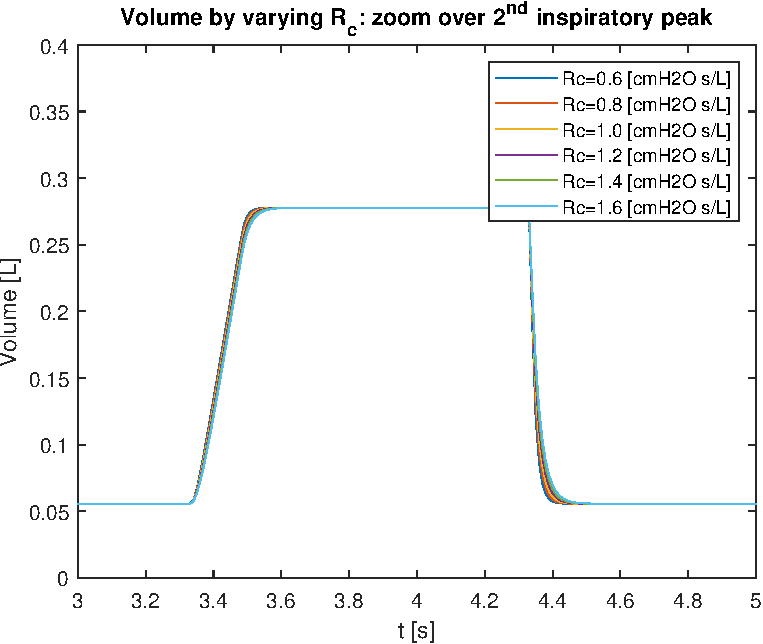
\includegraphics[width=0.95\linewidth]{../model/data_log/Rc_volume_zoom.pdf}
	\caption{}
\end{subfigure}\hfill
\caption{Volume con variazione della resistenza delle vie aeree superiori $R_c$ nel range $0.6\div 1$ [cmH\textsubscript{2}O s/L]. Volume nel tempo (a); zoom sul secondo periodo respiratorio (b). Si vede come il volume risente molto poco della variazione della resistenza.}
\label{fig:Rc_volume}
\end{figure*}


\begin{figure*}[t!]
	\begin{subfigure}{\linewidth}
		\centering
		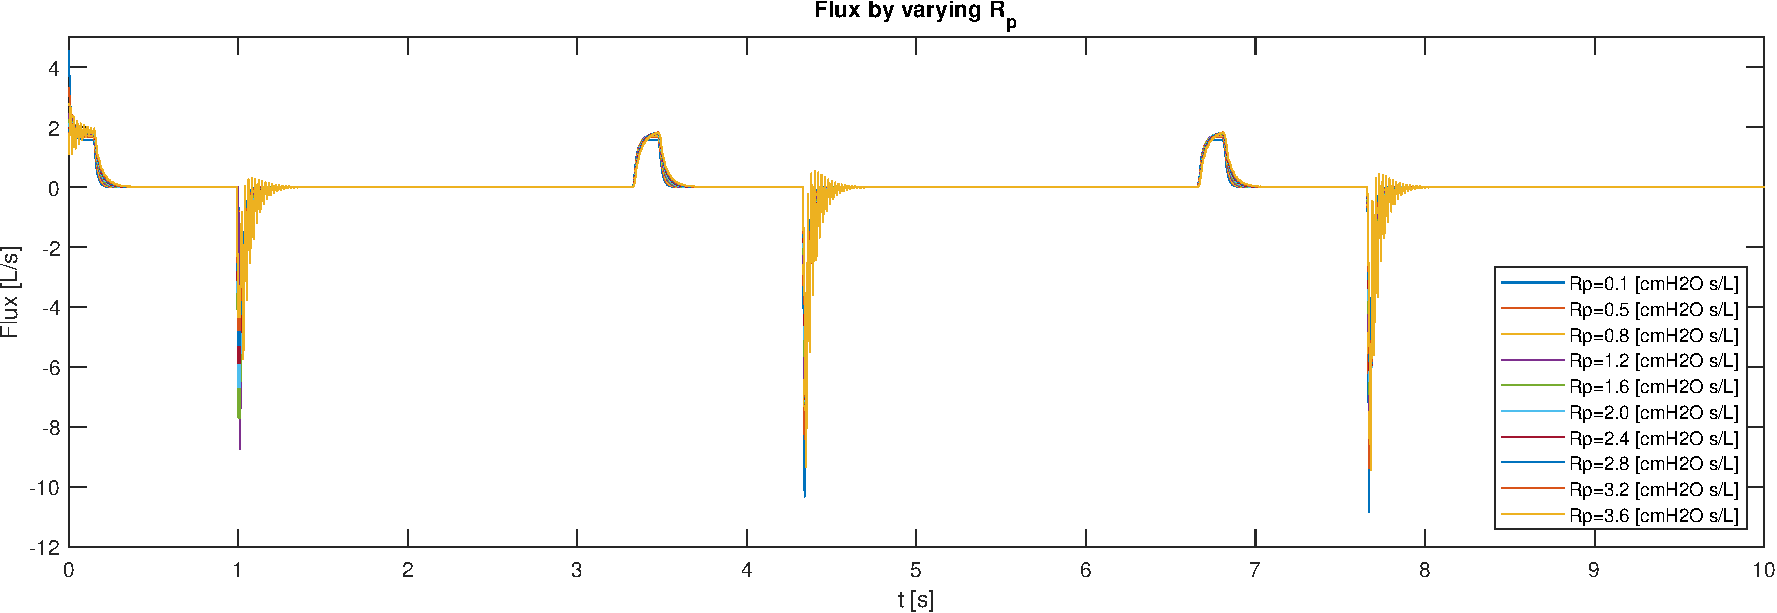
\includegraphics[width=0.95\linewidth]{../model/data_log/Rp_flux_total.pdf}
		\caption{}
	\end{subfigure}\hfill
	\begin{subfigure}{0.5\linewidth}
		\centering
		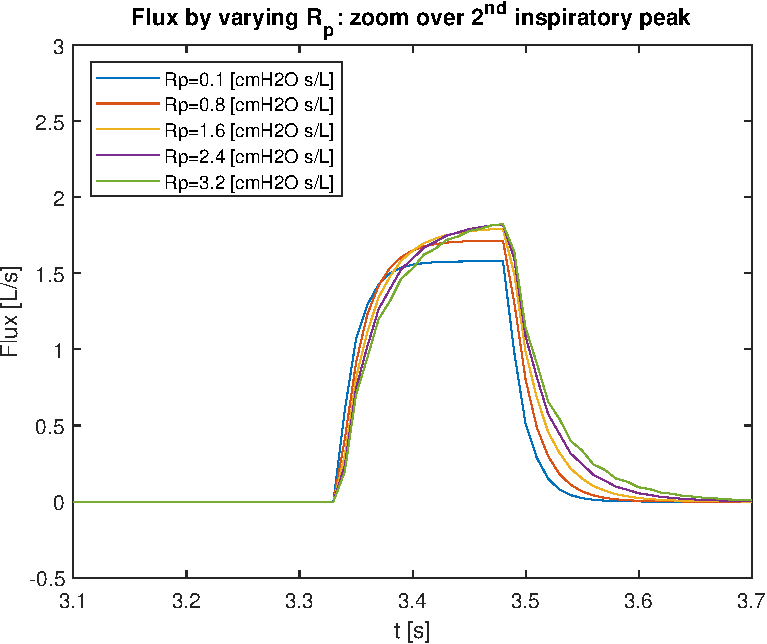
\includegraphics[width=0.95\linewidth]{../model/data_log/Rp_flux_zoom1.pdf}
		\caption{}
	\end{subfigure}\hfill
	\begin{subfigure}{0.5\linewidth}
		\centering
		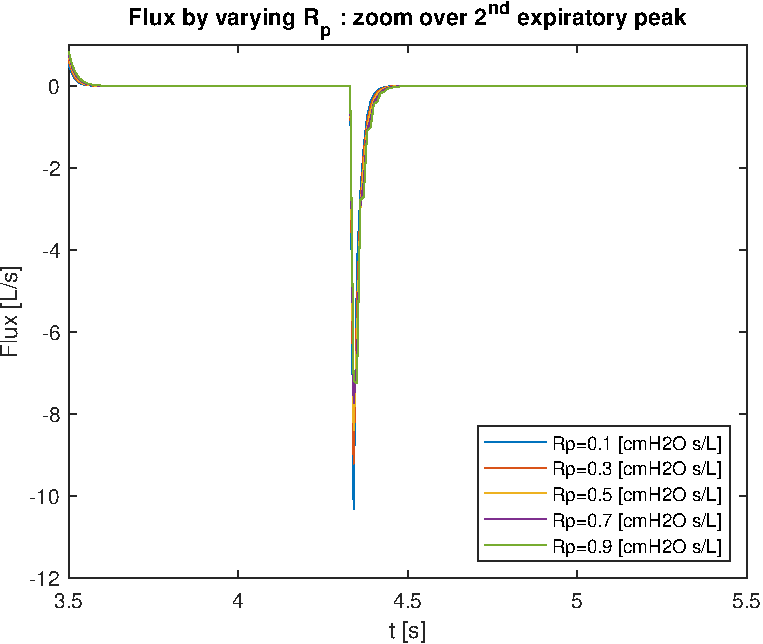
\includegraphics[width=0.95\linewidth]{../model/data_log/Rp_flux_zoom2.pdf}
		\caption{}
	\end{subfigure}\hfill
	\caption{Flusso con variazione della resistenza delle vie aeree inferiori $R_p$ nel range $0.1\div 3.6$ [cmH\textsubscript{2}O s/L]. Flusso nel tempo (a); zoom nel secondo periodo respiratorio sulla zona di influsso (b) ed efflusso (c). Si osserva un comportamento particolare, all'aumentare della resistenza aumenta il picco del flusso.}
	\label{fig:Rp_flux}
	\vspace{0.6 cm}
	\begin{subfigure}{0.7\linewidth}
		\centering
		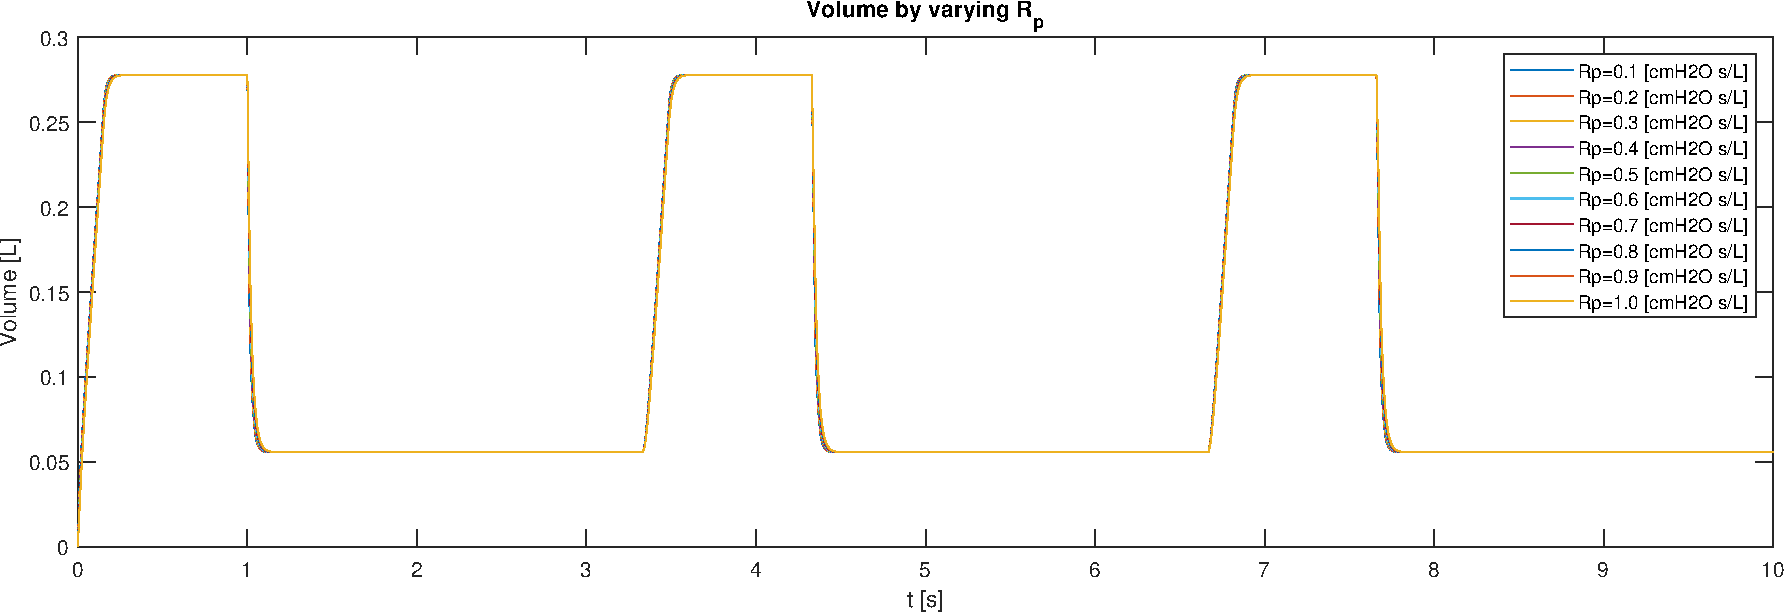
\includegraphics[width=0.95\linewidth]{../model/data_log/Rp_volume_total.pdf}
		\caption{}
	\end{subfigure}\hfill
	\begin{subfigure}{0.3\linewidth}
		\centering
		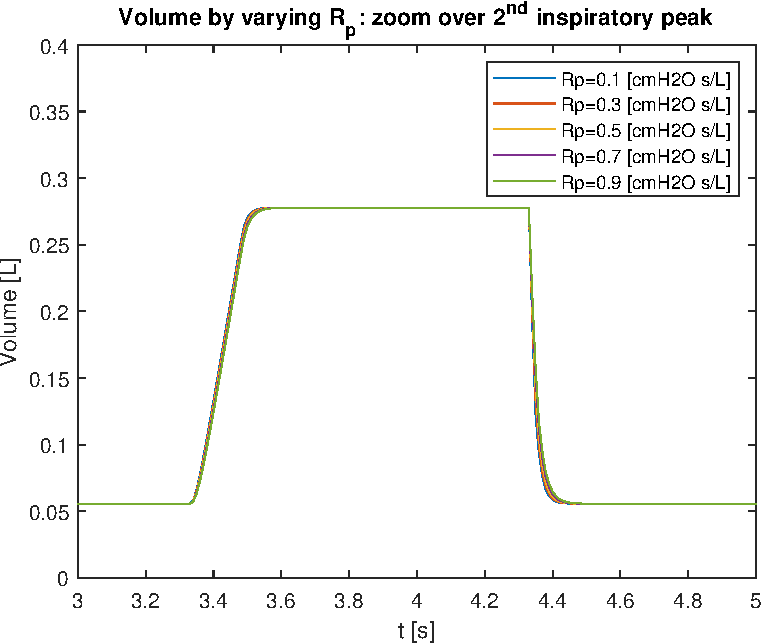
\includegraphics[width=0.95\linewidth]{../model/data_log/Rp_volume_zoom.pdf}
		\caption{}
	\end{subfigure}\hfill
	\caption{Volume con variazione della resistenza delle vie aeree inferiori $R_p$ nel range $0.1\div 3.6$ [cmH\textsubscript{2}O s/L]. Volume nel tempo (a); zoom sul secondo periodo respiratorio (b). Si vede come il volume risente molto poco della variazione della resistenza $R_p$. }
	\label{fig:Rp_volume}
\end{figure*}


\begin{figure*}[t!]
	\begin{subfigure}{\linewidth}
		\centering
		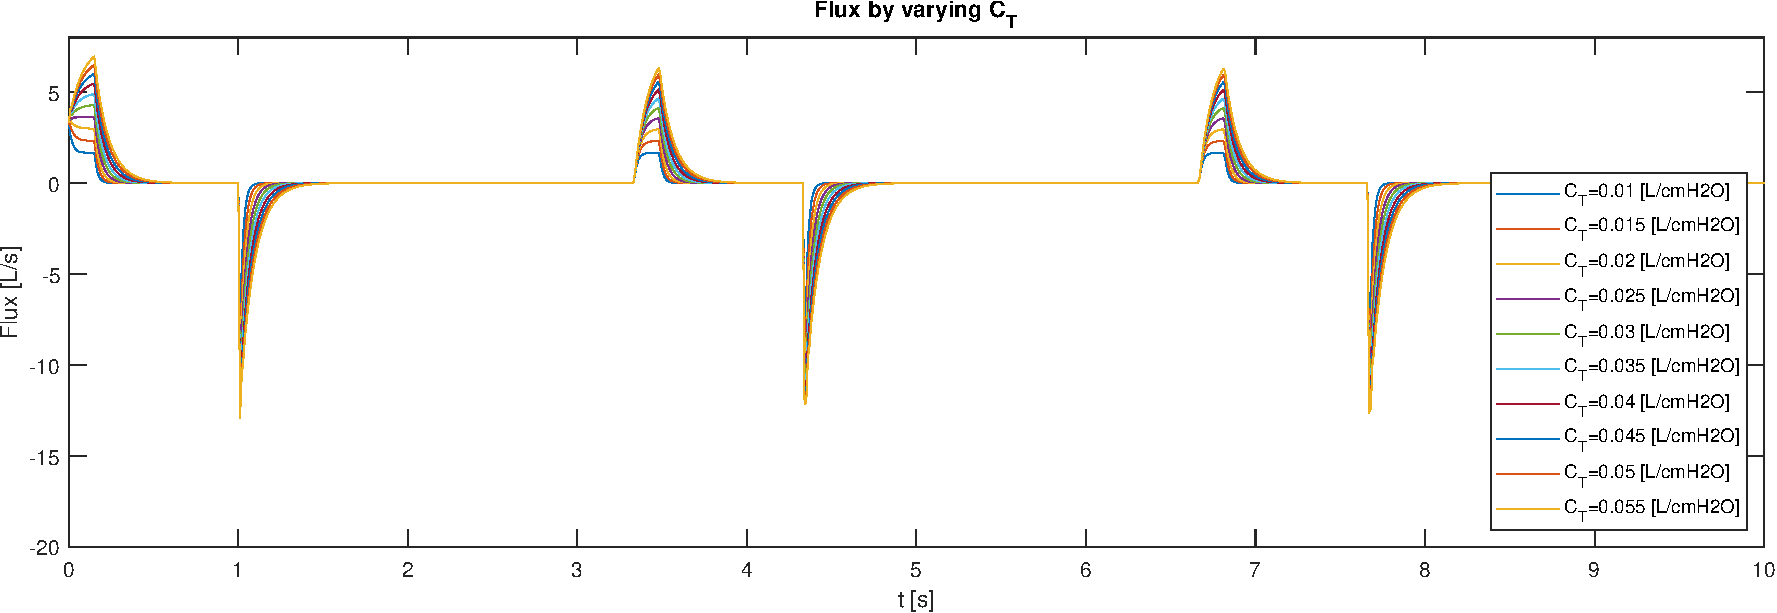
\includegraphics[width=0.95\linewidth]{../model/data_log/CwCL_flux_total.pdf}
		\caption{}
	\end{subfigure}\hfill
	\begin{subfigure}{0.5\linewidth}
		\centering
		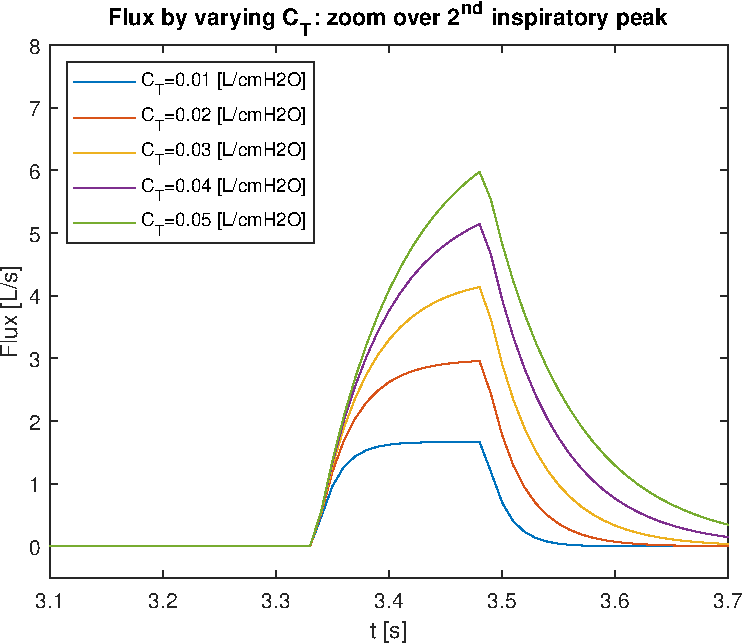
\includegraphics[width=0.95\linewidth]{../model/data_log/CwCL_flux_zoom1.pdf}
		\caption{}
	\end{subfigure}\hfill
	\begin{subfigure}{0.5\linewidth}
		\centering
		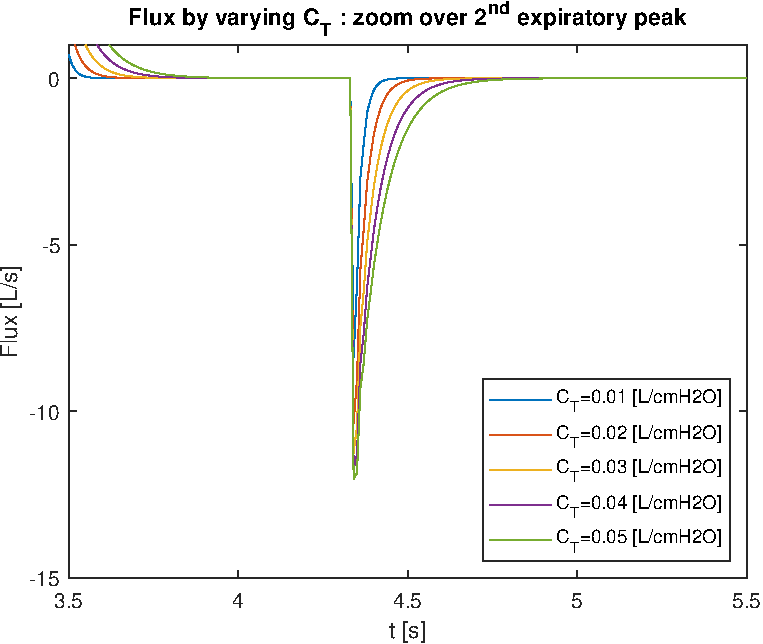
\includegraphics[width=0.95\linewidth]{../model/data_log/CwCL_flux_zoom2.pdf}
		\caption{}
	\end{subfigure}\hfill
	\caption{Flusso con variazione della compliance polmonare (serie di $C_w$ e $C_L$) nel range $0.005\div 0.050$ [L/cmH\textsubscript{2}O]. Flusso nel tempo (a); zoom nel secondo periodo respiratorio sulla zona di influsso (b) ed efflusso (c). Si osserva come il flusso è fortemente influenzato dalla compliance polmonare. L'aumento della capacità $C_T$ porta ad un forte aumento del picco di flusso.}
	\vspace{0.8 cm}
	\begin{subfigure}{\linewidth}
		\centering
		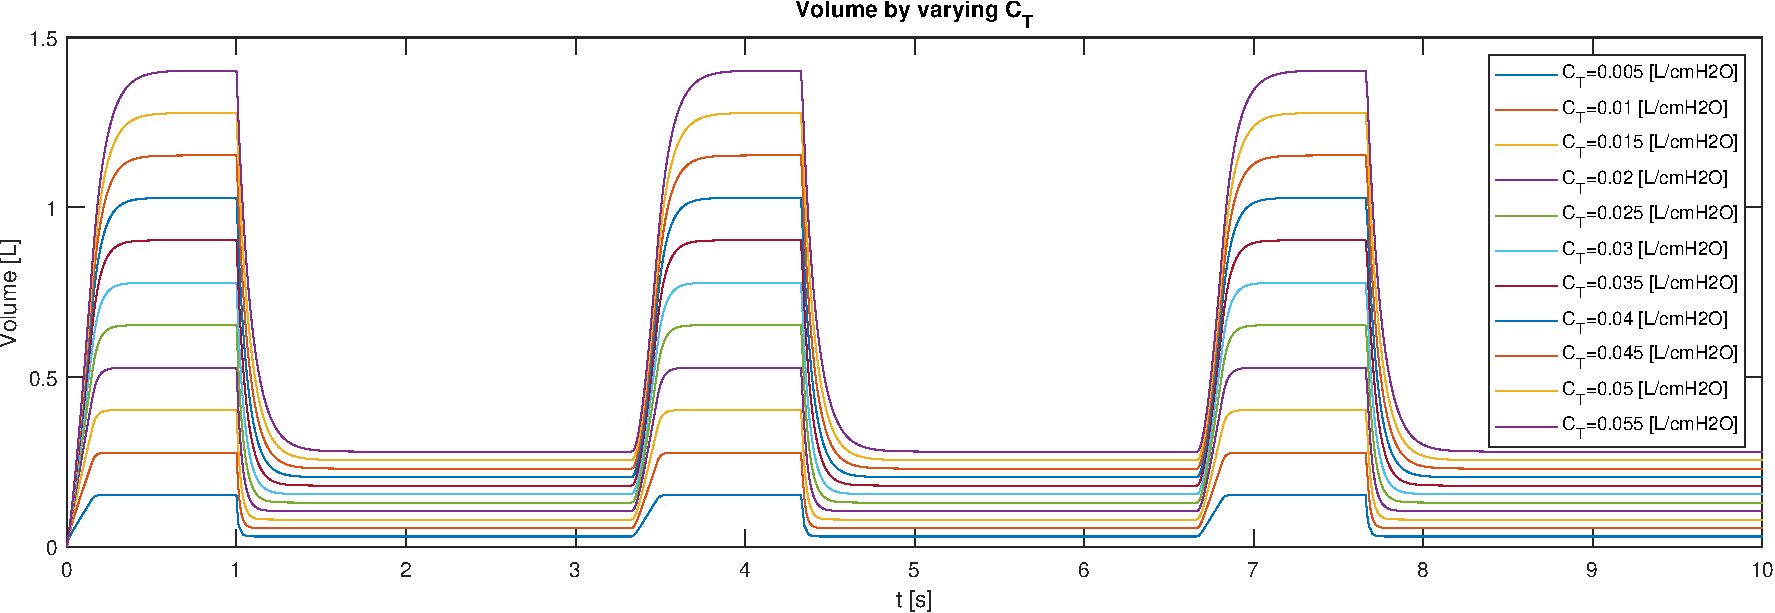
\includegraphics[width=0.95\linewidth]{../model/data_log/CwCL_volume_total.pdf}
	\end{subfigure}\hfill
	\caption{Volume con variazione della compliance polmonare (serie di $C_w$ e $C_L$) nel range $0.005\div 0.050$ [L/cmH\textsubscript{2}O]. Si vede come il volume è fortemente influenzato da $C_T$ ed in particolare come considerare valori troppo alti porta ad un ingresso di volume elevato che può risultare pericoloso per il polmone.}
\end{figure*}


\begin{figure*}[t!]
	\begin{subfigure}{0.5\linewidth}
	\centering
	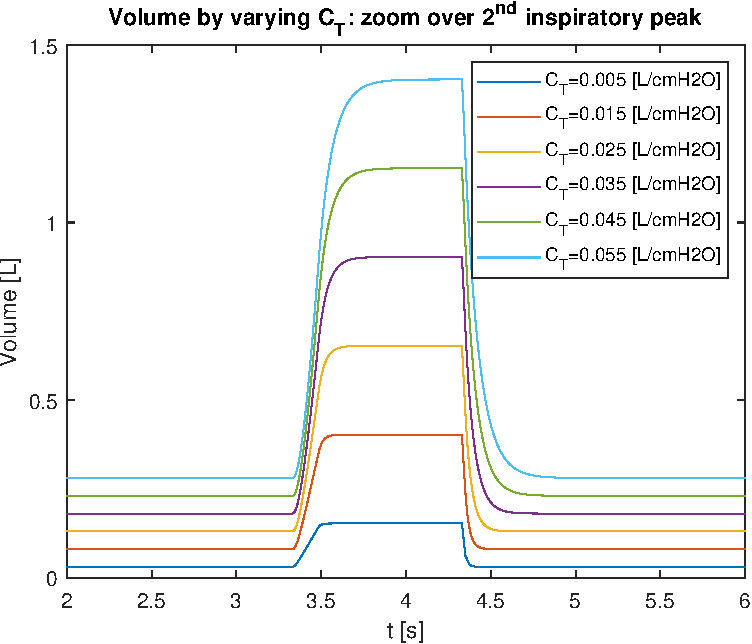
\includegraphics[width=0.95\linewidth]{../model/data_log/CwCL_volume_zoom.pdf}
	\caption{}
\end{subfigure}\hfill
	\begin{subfigure}{0.5\linewidth}
	\centering
	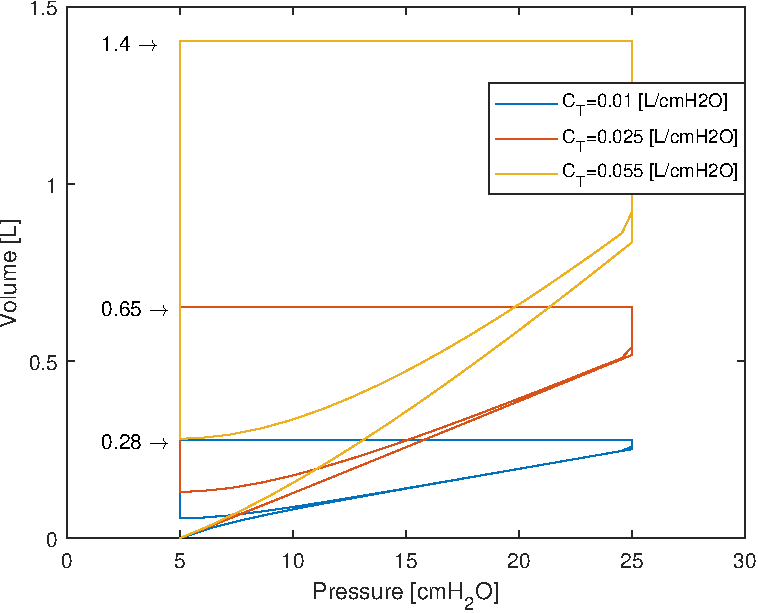
\includegraphics[width=0.95\linewidth]{../model/data_log/CwCL_PV.pdf}
	\caption{}
\end{subfigure}\hfill
	\caption{Volume con variazione della compliance polmonare (serie di $C_w$ e $C_L$) nel range $0.005\div 0.050$ [L/cmH\textsubscript{2}O]. Zoom sul secondo periodo respiratorio (a) e diagramma PV (b). Si vede come il volume è fortemente influenzato da $C_T$ ed in particolare come considerare valori troppo alti porta ad un ingresso di volume elevato che può risultare pericoloso per il polmone. Si vede, dal diagramma pressione-volume, come a parità di pressione può entrare un volume nettamente superiore a quanto dovrebbe essere garantito per rispettare i limiti fisiologici. }
\end{figure*}

\begin{figure*}[t!]
	\begin{subfigure}{0.6\linewidth}
		\centering
		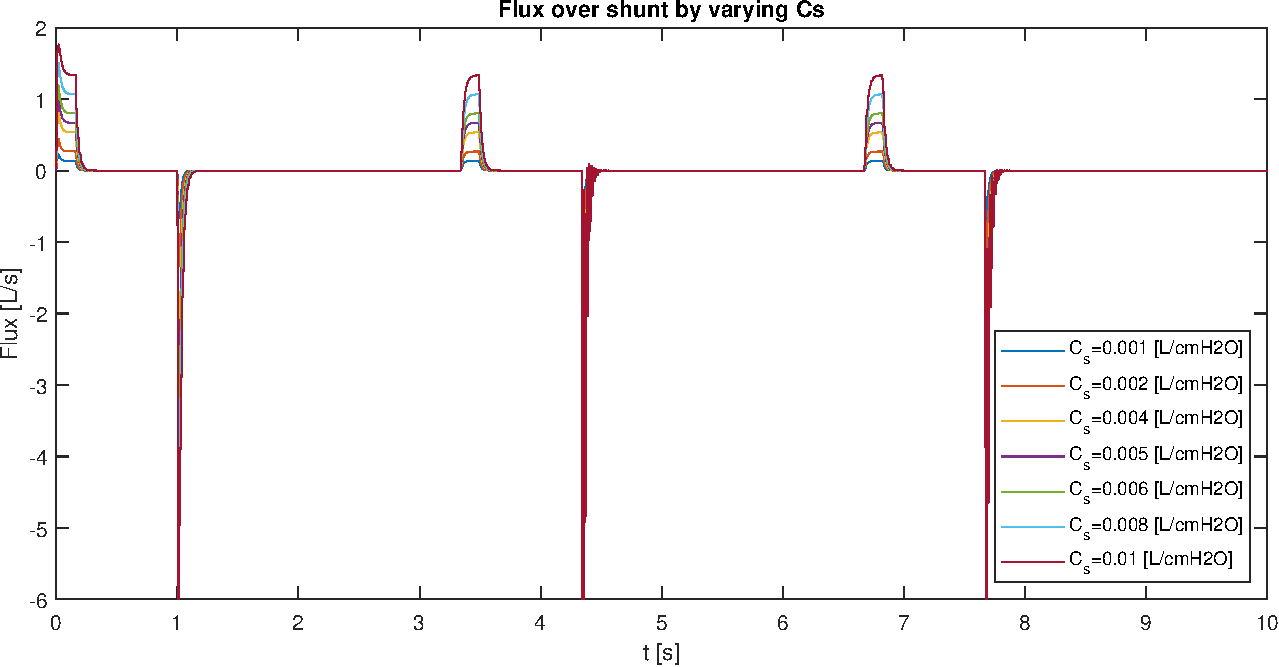
\includegraphics[width=0.95\linewidth]{../model/data_log/Cs_fluxCS.pdf}
		\caption{}
	\end{subfigure}\hfill
	\begin{subfigure}{0.4\linewidth}
		\centering
		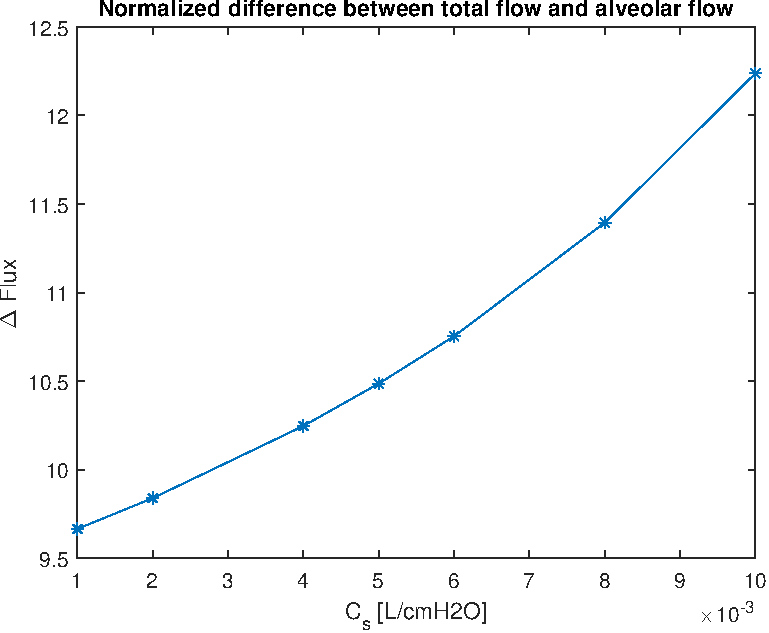
\includegraphics[width=0.95\linewidth]{../model/data_log/CwCL_deltaflux.pdf}
		\caption{}
		 \label{fig:flusso_shunt_delta}
	\end{subfigure}\hfill
	\caption{Flusso variando $C_s$ nel range $0.001\div 0.01$ [L/cmH\textsubscript{2}O] (a); norma della differenza di flusso tra shunt e alveoli (\cref{eq:shunt_Delta}) rispetto la variazione di $C_s$ (b). Si vede come aumentando la capacità di shunt un maggior flusso (e quindi volume) passerà per il ramo di shunt mentre il flusso complessivamente richiesto al ventilatore rimane quasi costante. Inoltre, più aumenta la $C_s$ più aumenta la differenza tra il flusso di shunt e quello alveolare e quindi il volume d'aria che effettivamente entra nel polmone si riduce. }
	\label{fig:flusso_shunt}
\end{figure*}

\begin{figure*}[t!]
	\begin{subfigure}{0.33\linewidth}
		\centering
		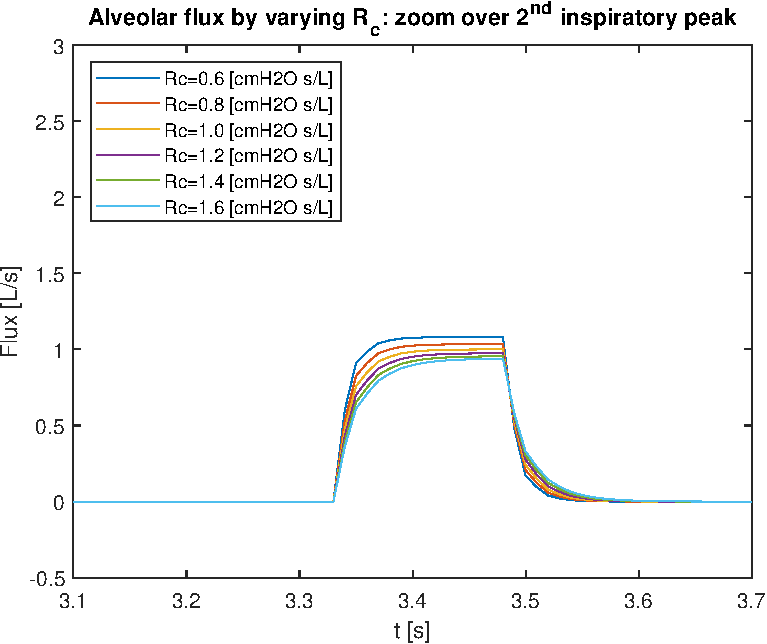
\includegraphics[width=0.95\linewidth]{../model/data_log/Rc_flux_alveolar_zoom.pdf}
		\caption{}
	\end{subfigure}\hfill
	\begin{subfigure}{0.33\linewidth}
		\centering
		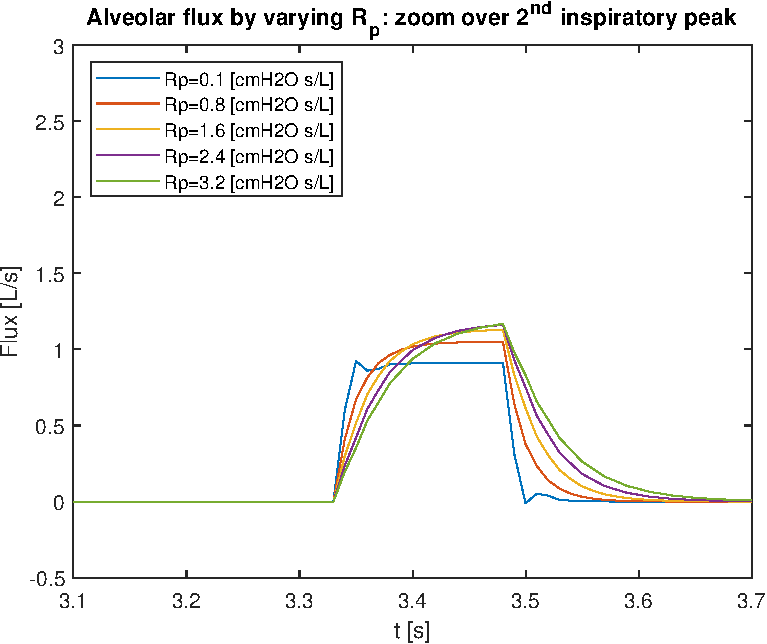
\includegraphics[width=0.95\linewidth]{../model/data_log/Rp_flux_alveolar_zoom.pdf}
		\caption{}
	\end{subfigure}\hfill
	\begin{subfigure}{0.33\linewidth}
	\centering
	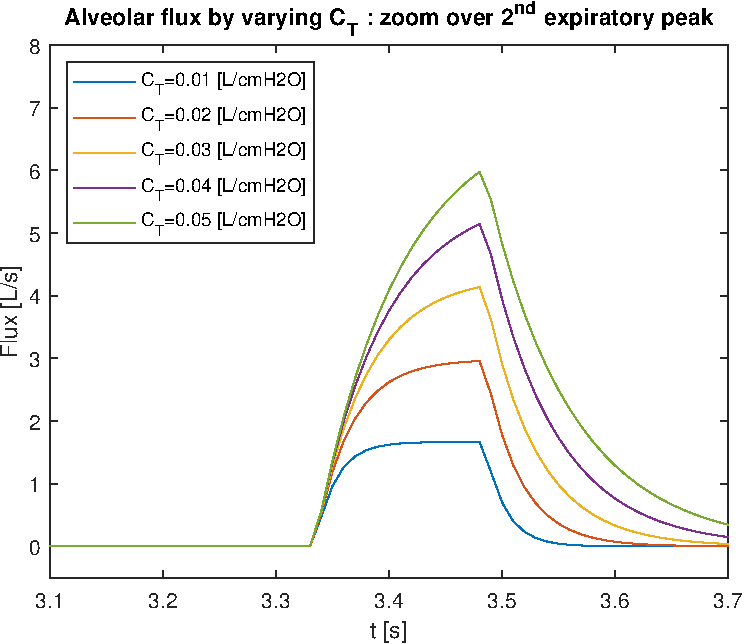
\includegraphics[width=0.95\linewidth]{../model/data_log/CwCL_alveolar_flux_zoom.pdf}
	\caption{}
\end{subfigure}\hfill
	\caption{Flusso alveolare rispetto le variazioni di $R_c$ (a), $R_p$ (b) e $C_T$ (c)}
\label{fig:flux_alveolar}
\end{figure*}



\subsection{Compliance polmonare}

Anche la compliance polmonare viene intaccata da alcune patologie.

Nelle bronco pneumopatie croniche ostruttive (BPCO) si verifica una riduzione della compliane polmonare.

Nel caso di edema polomonare cardiogeno (CPE) o non cardiogeno (ARDS) si verifica una riduzione della compliance fino a rispettivamente 0.044 L/cm H\textsubscript{2}O e 0.035 L/cm H\textsubscript{2}O \cite{milic-emili_basics_1999}.

A questo si aggiungono altri fattori che contribuiscono a ridurre la compliance polmonare quali atelettasia, pneumotorace, spostamento del tubo endotracheale e polmoniti \cite{grossbach_overview_2011}.
\\

La variazione della compliance influenza molto il volume d'aria che entra nei polmoni. In particolare, essendo tipicamente $C_s$ molto piccolo e quindi la quantità di flusso che viene diretto sulla porzione di shunt e non entra nei polmoni molto bassa, è possibile trascurare tale contributo e considerare il volume in ingresso nei polmoni come il volume erogato dal ventilatore.

Questo non è però vero nel caso in cui $C_s$ va ad aumentare. Infatti, come si può vedere dalla \cref{fig:flusso_shunt}, più aumenta $C_s$ più aumenta il flusso sul ramo shunt e più aumenta il divario tra il flusso totale (che invece rimane quasi costante con uno scarto medio inferiore a $10^{-3}$ [L/s]) e il flusso alveolare.

In figura \cref{fig:flusso_shunt_delta} viene riportata la norma della differenza tra il flusso erogato dal respiratore e quello alveolare, normalizzato rispetto al valore massimo. 

\begin{equation}
	\small{
\Delta \mathrm{Flux}={	\|\text{flusso su }C_s - \text{flusso alveolare}\|\over \max\left(\text{flusso su }C_s - \text{flusso alveolare}\right)}}
\label{eq:shunt_Delta}
\end{equation}

\subsection{Flusso alveolare}

Per avere la certezza della quantità d'aria effettivamente in ingresso nei polmoni e capace di effettuare scambi gassosi è necessario andare a leggere il valore di flusso sul ramo polmonare, ovvero sulla capacità $C_T$. 

Confrontando i valori di flusso alveolare \cref{fig:flux_alveolar}, al variare dei parametri del sistema, con le rispettive variazioni del flusso totale è possibile identificare quanto flusso effettivamente entra nel polmone. 

Nel caso della variazione delle resistenze la differenza tra i flussi rimane molto contenuta rispetto alla variazione della $C_T$ per la quale si vedono corrispondere quasi completamente le variazioni del flusso. Discorso diverso invece per la capacità di shunt per la quale corrisponde un aumento diretto del flusso di shunt a sfavore del flusso alveolare (\cref{fig:flusso_shunt}).

\section{Conclusioni}

I risultati mostrano come è necessario impostare correttamente sia i parametri della ventilazione sia stimare il comportamento del paziente. 

Variazioni dei parametri circuitali possono alterare il comportamento e la quantità d'aria richiesta al ventilatore. In particolare, il termine con maggior importanza è dato dalla sere delle capacità polmonari il cui aumento porta ad un aumento eccessivo dei volumi in ingresso fino a valori che possono risultare pericolosi per il paziente.

L'aumento della capacità di shunt tende ad aumentare il flusso deviato e quindi a togliere aria al polmone, nonostante il ventilatore immetta comunque più aria.

La variazione delle resistenze, nei range considerati, non si riflette tanto sulla variazione del flusso complessivo quanto sulla pendenza della sua forma d'onda.

La disponibilità di un modello di ventilatore polmonare accoppiato ad un modello di meccanica respiratoria permette di simulare l'interazione ventilatore-patologia e analizzare il metodo migliore di operare a seconda del parametro che viene deviato dalla patologia. 

%\pagebreak
\section*{Disponibilità dei dati}

Il materiale è disponibile alla repository online del progetto: \url{https://github.com/mastroalex/resp-mech-simulink}


\raggedbottom
%\pagebreak
\printbibliography[title=Riferimenti]
%\section*{References}


\clearpage
\onecolumn
\section*{Appendice}
\subsection*{Codice per la generazione della pressione di ingresso}
 \begin{figure*}[h!]
\begin{lstlisting}[language=matlab,basicstyle=\tiny\ttfamily,]
function y = fcn(t,flag_ventilation,breath_for_minute,tau_int,Paw,PEEP,T_insp)
	% % % to avoid error use the `odeN` solver !
	f=breath_for_minute/60; % breathing frequence in Hz
	% pressure diffrence from maximus value and PEEP
	DeltaPressure=Paw-PEEP; 
	A=0; % initialize output variable
	if flag_ventilation==1 % flag=1 for sine wave
		% sine wave from Khoo Physiological Control Sistem
		% amplitude peak-peak of 5 cmH2O
		amplitude=5;
		A=amplitude*sin(2*pi*f*t);  
	end
	if flag_ventilation==2 % flag=2 for perfect square wave
		dt=rem(t,(1/f)); % current time (of single period)
		period=1/f; 
		half_period=period/2; % duty cycle of 50 % by selecting half period
		if  dt<half_period % semi-period where the output is on
			amplitude=5;   % amplitude of 5 [cmH2O] 
			A=amplitude; % set the output constant
		end
		if dt>= half_period % semi-period where the output is zero
			A=0; % set the output to zero 
		end 
	end
	if flag_ventilation==3 % flag=3 for square wave with rise time tau
		period=1/f; 
		dt=rem(t,(1/f));  % current time (of single period)
		% the inspiratory time (where the output is on) is defined  usign percentage of total period with T_insp from ventilator GUI
		% also the rise time is defined using percentage of inspiratory time with tau_int from ventilator GUI
		insp_Time=(T_insp/100)*period; 
		tau=(tau_int/100)*insp_Time;
		if dt < tau % rise time
			% linear growth of the pressur with offset 
			A=DeltaPressure*(dt/tau)+PEEP; 
		end
		if  (dt>=tau) && (dt<insp_Time) % the pressure is max (square wave on)
			A=DeltaPressure+PEEP;
		end
		if dt>= insp_Time %the pressure is min (square wave off)
			A=PEEP;
		end 
	end
	y=A; % set the pressure wave as function output
end
\end{lstlisting}

\subsection*{Interfaccia grafica completa}

\centering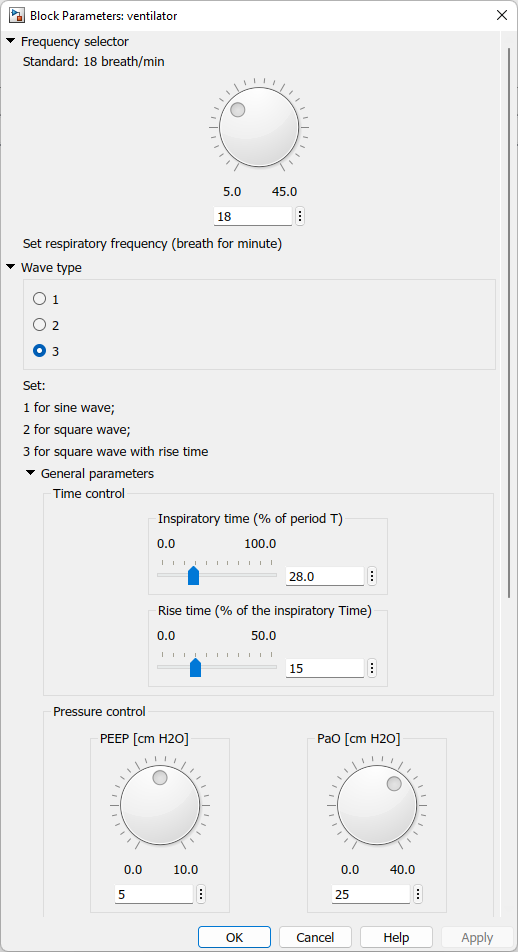
\includegraphics[angle=90,width=0.96\linewidth]{GUI.png}
	\caption{Interfaccia grafica completa del modello di ventilatore polmonare con possibilità di selezionare la forma d'onda, frequenza, pressione massima e minima, rise time e duty cycle.}
	\label{fig:interfaccia}
\end{figure*}

